\def\DevnagVersion{2.15}\documentclass[12pt,a4paper]{book}
\makeatletter\@openrightfalse\makeatother
% margins
\usepackage[left=35mm,top=25mm,right=25mm,bottom=25mm]{geometry}

% centering captions
\usepackage[justification=centering]{caption}
% mathematical expressions
\usepackage{mathtools}
\usepackage{textcomp}
\usepackage{caption}
\usepackage{pdfpages}
\usepackage{subcaption}
\usepackage{devanagari}
\usepackage{multirow}
\usepackage{amsmath}
\everymath{\displaystyle}

%\usepackage{algorithm2e}
\usepackage{pdfpages}

% to write the date in the desired format
\usepackage{datetime}
\usepackage{graphicx}

\usepackage{hyperref}

% for doublespacing singlespacing etc.
\usepackage{setspace}

\graphicspath{{img/}}

\newdateformat{monthyear}{\monthname[\THEMONTH], \THEYEAR}
\newcommand*\rfrac[2]{{}^{#1}\!/_{#2}}

\def\title{Distributed Semantics: Vector Models for NLP tasks in Hindi}
\def\degree{Master of Technology}
\def\author{Pranjal Singh}
\def\rollno{10327511}
\def\advisor{Dr. Amitabha Mukerjee}
\def\department{Department of Computer Science and Engineering}
\def\institute{Indian Institute of Technology Kanpur}

\hypersetup{
	bookmarks=true,
	bookmarksopen=true,
	bookmarksopenlevel=0,
	bookmarksnumbered=true,
	hypertexnames=false,
	colorlinks=true,
	linkcolor={black},
	citecolor={black},
	urlcolor={black},
	breaklinks=true,
	pdfauthor={\author},
	pdftitle={\title}
}

\begin{document}
	\frontmatter
	\begin{titlepage}
	\pagestyle{empty}
		
	\begin{center}
		\huge{\textbf{\title}}\\
	\end{center}

	\vspace{0.5in}
	\begin{center}
		\large\textit{A Thesis Submitted \\ in Partial Fulfilment of the Requirements \\ for the Degree of}\\
		\vspace{0.2in}
		\large\textbf{\degree}\\
	\end{center}
	
	\vspace{0.3in}
	\begin{center}
		\Large\textit{by}\\
		\Large\bf{\author}\\
		\Large{Roll No.: \rollno}\\
	\end{center}
	
	\vspace{0.5in}
	\begin{center}
		\Large\textit{under the guidance of}\\
		\Large\bf{\advisor}\\
		\vspace{0.35in}
	\end{center}
	
	\vfill
	\begin{center}
		\begin{figure}[htbp]
			\centering
			
\includegraphics[width=5cm]{iitkblue.eps}
		\end{figure}

		\vspace{0.2in}
		\large{\department}\\
		\vspace{0.1in}
		\large{\institute}\\ 
		\vspace{0.03in}
		\Large{\monthyear\today}
	\end{center}
	
\end{titlepage}

	
	\thispagestyle{empty}
	\pagestyle{plain}
%	\cleardoublepage
	\vspace*{1.0in}
\begin{center}
\begin{large}
{\bf CERTIFICATE}
\end{large}
\end{center}
\vskip 2cm
%It is certified that the work contained in this thesis entitled \\``{{\textit{\title, \subtitle.}}}'',\\ by {{\textit{Asheesh Agrawal (Roll No. Y8127139)}}}, has been carried out under my \\supervision and that this work has not been submitted elsewhere for a degree.
It is certified that the work contained in this thesis entitled ``{{\textit{\title}}}'', by {{\textit{\author \hspace{1mm} (Roll No. \rollno)}}}, has been carried out under my 
supervision and that this work has not been submitted elsewhere for a degree.
\vskip 1in
\begin{flushleft}
		\hspace*{5.8cm}{\hrulefill}\\
		\hspace*{5.8cm}(\advisor)\\
		\hspace*{5.8cm}\department,\\ 
		\hspace*{5.8cm}\institute\\
		\hspace*{5.8cm}Kanpur - 208016
\end{flushleft}
\monthyear\today
%	
\includepdf{certificate_signed.pdf}

	\pagenumbering{roman}
	\pagestyle{plain}
	\setcounter{page}{2}
	\addcontentsline{toc}{chapter}{Abstract}
	
	%\onehalfspace
	\doublespacing
	\cleardoublepage

\begin{center}
	\huge{\textbf{Abstract}}
\end{center}

In recent years, distributional semantics or vector models for words and documents have been proposed to capture both the syntactic and semantic similarities. Since these are language free models and can be obtained in an unsupervised manner, they are of interest for under-resourced languages such as Hindi and many more other languages.
Language free models are generic and, in recent years, have developed the capability of performing various NLP tasks efficiently. Their capability of being invariant for different languages has attracted the attention of various researchers. We have developed such a language free model using distributional semantics and traditional language representation methods and achieved better results than language models. Their better time complexity has led us to experiment with various factors and parameters leading us to the claim that different languages and domains have different optimal parameters and different properties.

We test the efficacy of such an approach for many things and especially Hindi, first by a subjective overview which shows that a reasonable measure of word similarity seems to be captured quite easily.  We then apply it to the sentiment analysis for many English review datasets including IMDB and two small Hindi databases from earlier work and our own built dataset of Hindi movie reviews. 
We have gone a step ahead with document vectors and built new features merged with various models to achieve state-of-the art results in sentiment classification on classical IMDB movie review dataset achieving an accuracy of 94.19\%(improvement of 1.61\% over previous best). We also implement an ensemble model which boosts our accuracy by about 0.5\% using recurrent neural network.
We demonstrate the language free aspects by developing a huge increment on results for Hindi. We also propose that dimensionality reduction techniques such as ANOVA-F and PCA are of great help to reduce noise and boost accuracy of our models.

In order to handle larger strings from the word vectors, several methods - additive, multiplicative, or tensor neural models, have been proposed.  Here we propose weighted additive average technique, which results in an impressive accuracy gain on state of the art by 12\% (from 80\%) for two hindi review datasets.  The results suggest that it may be worthwhile to explore such methods further for Indian languages.\\


	\cleardoublepage

\vspace*{\fill}
\begin{center}
	{\it Dedicated to my Parents, Brother and Friends for their love and support}
\end{center}
\vspace*{\fill}

	\cleardoublepage

\begin{center}
	{\huge{\textbf{Acknowledgement}}}
\end{center}

I would like to take this opportunity to thank the people who have helped me in preparation of this thesis.

First of all, I would like to express my sincere gratitude towards my thesis supervisor, Dr. Amitabha Mukerjee, for his  constant support and encouragement. I am grateful for his patient guidance and advice which gave a proper direction to my efforts. I am grateful to him for providing me ample freedom to choose a topic of my interest and deciding how to pursue it.

I thank the Department of Computer Science and Engineering, IIT Kanpur, for providing the necessary infrastructure and a congenial environment for research work. I thank Tomas Mikolov for making the code of word2vec and sentence2vec publicly available.

I am also thankful to all my friends and specially wingmates (chaman, ladha, chotu, anshu, lassu, mm, baba, aryan, deo and few more) who have made my stay at IIT Kanpur most enjoyable and who in general gave me strength and hope whenever I required.
Last, but not the least, I thank my parents for always being there for me.

\vskip 4mm
\begin{flushright}
\textit{\textbf{\author}}
\end{flushright}

	
	\doublespacing
	\setcounter{secnumdepth}{3}
	\setcounter{tocdepth}{1}
	\tableofcontents
	\listoftables
	\addcontentsline{toc}{chapter}{List of Tables}
	\listoffigures
	\addcontentsline{toc}{chapter}{List of Figures}
%	\listofalgorithms
%	\addcontentsline{toc}{chapter}{List of Algorithms}
	
	\mainmatter
	\doublespacing
	\pagenumbering{arabic}
	\pagestyle{myheadings}
	
	\chapter{Introduction}
Over a period of nearly a millennium, Indian grammarians have been trying to find whether sentence meaning accrues by combining word meanings, or whether words gain their meanings based on the context they appear in \cite{Matilal:90}.  The former position, that meaning is {\em compositional}, has been associated with the fregean enterprise of semantics, whereas recent models, building on large corpora of text (and associated multimedia) a large degree of success has accrued to models that attempt to model word meaning based on their linguistic context (e.g. ~\cite{Landauer:97}). The latter line has resulted in strong improvements in several NLP tasks using word vectors~\cite{Collobert:08,Turian:10,Mikolov:13a,Socher:13}. Recently, the introduction of sentence/document vectors have achieved very good results in various NLP task~\cite{Le:14}. The advantage of these approaches is that they can capture both the syntactic and the semantic similarity between words/documents in terms of their projections onto a high-dimensional vector space; further, it seems that one can tune the privileging of syntax over semantics by using local as opposed to large contexts~\cite{Huang:12}. 

For resource-poor languages, these approaches have the added lure that many of these methods are completely unsupervised and work directly with large raw text corpora, thus avoiding contentious issues such as deciding on a POS-tagset, or expensive human annotated resources such as treebanks.  For Indian languages which are highly inflected, stemming or identifying the lemma is another problem
which such models can overcome, provided the corpus is large enough. Nonetheless, this approach remains under-explored for Indian languages. At the same time, it must be noted that many approaches seek to improve their performance by combining POS-tags and even parse tree structures into the models for higher accuracies in specific tasks~\cite{Socher:13}. 

Vector models for individual words are obtained via distributional learning, the mechanisms for which varies from document-term matrix factorization~\cite{Landauer:97}, various forms of deep learning~\cite{Collobert:08,Turian:10,Socher:13}, optimizing models to explain co-occurrence constraints ~\cite{Mikolov:13a,Pennington:14},etc. Once the word vectors have been assigned, similarity between words can be captured via cosine distances. The same models have been extended(\cite{Le:14}) with new variables to build vector models for sentences and documents. These models include the essence of individual words as well as their relative order in terms of sentence vector which was earlier absent in word vectors.

\cite{Chirawichitchai:14}
\cite{Sharma:14}
One problem in this approach is that of  combining the word vectors into larger phrases. In past work, inverse-similarity weighted averaging appears to work to some extent even for complex tasks such as essay grading \cite{Landauer:03}, but multiplicative models (based on a reducing the tensor products of the vectors) appears to correlate better with human judgements~\cite{Mitchell:08,Socher:13}.
Another complexity in composition is that composing words across phrasal boundaries are less meaningful than composing them within a phrase - this has led to models that evaluate the nodes of a parse tree, so that only coherent phrases are evaluated~\cite{Socher:13}. The results reported here, are based on applying the Skip-Gram  model~\cite{Mikolov:13b} to Hindi. 

\subsection{Sentiment Analysis}
In order to evaluate the efficacy of the model, we apply it to the task of sentiment analysis. Here the problem is that of identifying the polarity of sentences (Liu et al. 2012); for example: 
\begin{itemize}
\item Positive: {\dn rA\8{m} n\? khAnF kF r\327wtAr khF{\qva} Tmn\? nhF{\qva} dF} [Ramu didn't allow the pace of the story to subside]
\item Negative: {\dn pd\?{\qvb} pr EdKAyA jA rhA KO\327w Esn\?mAGr m\?
nhF{\qva} psr pAtA} [The horror shown on the screen didn't reach the theater]
\end{itemize}

This is a problem that has attracted reasonable attention in both Hindi and English (see section~\ref{sec:related}). 

In this work, we first learn a distributional word vector model as well as sentence vector model based on the wikipedia corpus as well as the sentiment corpus, and then we use this to discern the polarities on the existing corpora of movie and product reviews. To our own surprise, we find that even a simple additive composition model improves the state of the art in this task significantly (a gain of nearly 10\%). With weighted additive composition, the gain is more than 2\% beating the state-of-the-art in Hindi(\cite{Singh:15}). When used for the much better-researched, larger datasets of English the system does respectably, but well behind the very best models that attempt more complex composition models. So the question arises as to whether the very significant gains in Hindi are due to some quirk in the dataset, or could it be that Hindi word vectors are particularly informative,
e.g. owing to more highly inflected nature of its surface forms.  Also, if the results are not corpus-specific, it also raises the possibility that word vector methods may result in significant gains in
other similar problems for Hindi. 

For example, the sentences below give a brief idea of what positive and negative sentiment means.
\begin{itemize}
\item Positive: {\dn yh EPSm aQCF h\4}
\item Negative: {\dn yh smAn b\7{h}t KrAb h\4}
\end{itemize}
\footnotetext{en.wikipedia.org/wiki/List\_of\_languages\_by\_number\_of\_native\_speakers}
Majority of the existing work in this field is in English (Pang and Lee, 2008).

We then go a step ahead to build a model using document vectors along with tfidf and ensemble techniques to achieve state-of-the-art result on IMDB movie review dataset achieving a significant improvement over the previous best. We have got an accuracy of 94.19\% by using an ensemble method merged with recursive neural network to show the excellency of generative models merged with discriminative ones.
Our model uses concatenation of average word vectors, sentence vectors and tf-idf to build informative document vectors which constitute a feature set for our SVM classier. We have used skip-gram model (Mikolov et al., 2013b) for building word vectors because deep network model of Collobert et al.(2008) takes too much time for training. Also the word embeddings obtained by them are not as good as those obtained by Mikolov et al.(2013b). \\
For Hindi, we have experimented with tf-idf and weighted average word vectors for building our feature set. Our model shows slight improvement in performance if we filter out certain corpus based stop words. This is a first attempt to use word vectors for sentiment analysis in Hindi. Word vectors capture both semantic and syntactic information for a given corpus. Words which are semantically and syntactically related tend to be closer in high-dimensional space.\\

\section{The Problem}
The problem undertaken in this thesis is to use Distributional Semantics for under-resourced languages such as Hindi to cater to a very significant NLP task of sentiment analysis. We also took the task of using distributional semantics with various forms of composition of vectors and even features to build good models for English as well. We have also laid a systematic background to the problem of context size and how it is related to syntactic and semantic similarity in text. 

\section{Contributions of this Thesis}
There are three main contributions of this thesis:
\begin{itemize}
\item We have successfully applied distributional models for Hindi and achieved state-of-the-art results on standard corpus of product and movie reviews. As a result, we have successfully published our work in regICON-2015 organized at IIT-BHU.
\item We have also compiled a corpus in Hindi containing around 700 Movie Reviews which is the largest corpus in Hindi in this domain. For reference,we will call it as \emph{700-Movie reviews} dataset.
\item We have achieved state-of-the-art results on IMDB Movie Review dataset(94.19\%) and have beaten the previous best by over 1.6\% in terms of accuracy.
\end{itemize}

\section{Organization of this Thesis}
The rest of this thesis is organized as follows. Chapter \ref{sec:related} presents related work done and discusses the various background work that one must be acquainted with in order to understand the work presented. Chapter \ref{sec:data} discusses the data sources and presents the statistics of each dataset. Chapter \ref{sec:dimensionality_reduction} gives an overview of dimensionality reduction techniques and how we have successfully applied them on vectors of our Hindi corpus to achieve very good results. Chapter \ref{sec:experiment} then discusses in detail the implemented methods and algorithms. Chapter \ref{sec:result} presents a summary of the results that was achieved. Chapter \ref{sec:conclusion} presents concluding remarks to our work and talks about what can be done further.

	\chapter{Related Work and Background}
\label{sec:related}
Sentiment analysis is a well-known research area in NLP today (see reviews in~\cite{Liu:12} and Pang et al. (2008), and also
challenge in SemEval-2014).  Early work on movie review sentiments achieved an accuracy of 87.2\% (Pang et al. 2004) on a dataset that discarded objective sentences and used text categorization techniques
on the subjective sentences. Le and Mikolov (2014) use word vector models and obtain 92.6\% accuracy on IMDB movie review dataset.
They used distributed bag-of-words model, which they call as \emph{paragraph vector}. More difficult challenges involve short texts with nonstandard vocabularies,as in twitter.  Here, some authors focus on building extensive feature sets (e.g. Mohammad et al.(2013); F-score 89.14). \\
% WANG IS NOT BEING REFERRED TO
Wang et al. (2014) propose a word vector neural-network model, which takes both sentiment and semantic information into account. This word vector expression model learns word semantics and sentiment at the same time as well as fuses unsupervised contextual information and sentence level supervised labels.

Neelakantan et al.(2015)\cite{Neelakantan:14} took word vector models to next level where they proposed multiple embeddings per word. Nearly all the work before this assumes a single vector per word
type—ignoring polysemy and thus jeopardizing their usefulness for downstream tasks. The authors present an extension to the Skip-gram model that efficiently learns multiple embeddings per word type. It differs from recent related work by jointly performing word sense discrimination and embedding learning, by non-parametrically estimating the number of senses per word type, and by its efficiency and scalability. They achieve state-of-the-art results in the word similarity in context task and demonstrate its scalability by training with one machine on a corpus of nearly 1 billion tokens in less than 6 hours.

Since most sentiment analysis is oriented towards semantics, and one may bypass the syntactic
processing which remains poor for Hindi. Methods that have been used are largely based on assigning a sentiment effect for individual words, and then combining these in some manner to come up with an overall sentiment for the document. Such methods ignore word order and have been criticized since the import of a sentence can change completely simply by re-arranging the words, though the sentiment evaluation remains the same. Several groups have attempted to improve the situation by modeling the composition of words into larger contexts \cite{Le:14,Socher:13,Johnson:14,Baroni:14}.

However, most of the work on sentiment analysis in Hindi has not attempted to form richer compositional analyses.   For the type of corpora used here, the best results, obtained by combining a sentiment lexicon with hand-crafted rules (e.g. modeling negation and "but" phrases), reach an accuracy of 80\%~\cite{Mittal:13}.

There has been limited work on sentiment analysis in Hindi -- see review in
~\cite{Medagoda:13}, who surveys sentiment analysis in non-English languages). Joshi et al. (2010) compared three approaches: In-language sentiment
analysis, Machine Translation and Resource Based Sentiment Analysis. By using WordNet linking, words in English SentiWordNet were replaced by equivalent Hindi words to get H-SWN. The final accuracy achieved by them is 78.1\%.

\cite{Bakliwal:12}
traversed the WordNet ontology to antonyms and synonyms 
to identify polarity shifts in the word space. Further
improvements were achieved by using a partial stemmer (there is no good
stemmer / morphological analyzer for Hindi), and focusing on 
adjective/adverbs (45 + 75 seed words given to the system); their 
final accuracy was 79.0\% for the product review dataset. 
Mukherjee et al. (2012) presented the inclusion of discourse markers in a bag-of-words model and how it improved the sentiment classification accuracy by 2-4\%.  % <--- NOT HINDI
Mittal et al. (2013) incorporate hand-coded rules dealing with negation and discourse relations and extend the HSWN lexicon with more opinion words.  Their algorithm achieves  80.2\%
accuracy on classification of movie reviews on a separate dataset.\\

\cite{Mikolov:10} presents new recurrent neural network based language model which has found vital application in various NLP tasks as well. They provide ample empirical evidence to suggest that connectionist language models are superior to standard n-gram techniques, except their high computational (training) complexity. The model has also been extended to speedup training time by few optimizations.(More details in \ref{sec:rnn}).

The algorithms and data structures used in this thesis have been introduced and discussed below.
\section{Word-Vectors and Representations}
\subsection{Skip-Gram}
\label{sec:skipgram}
Mikolov et al. (2013b) proposed two neural network models for building word vectors from large unlabeled corpora; Continuous Bag of Words(CBOW) and Skip-Gram.  In the CBOW model, the context is the input, and one tries to learn a vector for the central word; in Skip grams, the input is the target word and one tries to guess the set of contexts.  The Skip gram was found to perform better on smaller corpora, and here we have focused on this model for building our word vectors. The model uses each current word as an input to a log-linear classifier with continuous projection layer, and predict words within a certain range before and after the current word. The objective is to maximize the probability of the context given a word within a language model:

\begin{center} $p(c|w;\theta)=\frac{\exp^{v_c.v_w}}{\sum_{c' \in C}\exp^{v_c.v_w}}$ \end{center}
where $v_c$ and $v_w$ $\in$ $R^d$ are vector representations for context $c$ and word $w$ respectively. $C$ is the set of all available contexts. The parameters $\theta$ are $v_ci$, $v_wi$ for $w \in V$, $c \in C$, $i \in 1,....,d$ (a total of $|C| \times |V| \times d$ parameters).\\

The weights between the input layer and the output layer can be represented by a $V \times N$ matrix \textbf{W}. Each row of \textbf{W} is the $N$-dimension vector representation $v_w$ of the associated word of the input layer.Given a word, assuming $x_k=1$ and $x_{k'}=0$ for $k' \neq k$, then
\begin{center}
$h=x^TW=W_{(k,.)}:=v_{w_I}$
\end{center}
which is essentially copying the $k$-th row of \textbf{W} to \textbf{h}. $v_{w_I}$ is the vector representation of the input word $w_I$.

From the hidden layer to the output layer, there is a different weight matrix \textbf{W'}=$\{w_{ij}^{'}\}$ which is a $N \times V$ matrix. Then we can use soft-max, a log-linear classification model, to obtain the posterior distribution of words, which is a multinomial distribution.\\
On the output layer, instead of outputting one multinomial distribution, we are outputting C multinomial distributions. Each output is computed using the same hidden$\rightarrow$output matrix.
\begin{center}
$p(w_{c,j}=w_{O,c}|w_I)=y_{c,j}=\frac{exp(u_{c,j})}{\sum_{j'=1}^{V}exp(u_{j'})}$
\end{center}
where $w_{c,j}$ is the $j$-th word on the $c$-th panel of the output layer; $w_{O,c}$ is the actual $c$-th word in the output context words; $w_I$ is the only input word; $y_{c,j}$ is the output of the $j$-th node on the $c$-th panel of the output layer; $u_{c,j}$ is the net input of the $j$-th node on the $c$-th panel of the output layer.
Because the output layer panels share the same weights, thus
\begin{center}
$u_{c,j}=u_j=v`_{w_j}^T.h$, for $c=1,2...,C$
\end{center}
where $v'_{w_j}$ is the output vector of the $j$-th word in the vocabulary, $w_j$, and also $v'_{w_j}$ is taken from a column of the hidden$\rightarrow$output weight matrix, \textbf{W'} .

The loss function is
\begin{center}
E = -$\log p(w_{O,1},w_{O,2},....,w_{O,C}|w_I)$\\
=-$\log \prod_{c=1}^{C}\frac{exp(u_{c,j_{c}^{*	}})}{\sum_{j'=1}^{V}exp(u_{j'})}$\\
=-$\sum_{c=1}^{C} u_{j_{c}^{*}}+C.\log \sum_{j'=1}^{V}exp(u_{j'})$
\end{center}
where $j_{c}^{*}$ is the index of the actual $c$-th output context word in the vocabulary.

After taking the necessary derivatives, the update equation for the hidden$\rightarrow$output weight matrix, \textbf{W'},
\begin{center}
$w'{ij}^{(new)}=w'{ij}^{(old)}-\eta .EI_j.h_i$
\end{center}
or,
\begin{center}
$v'{w_j}^{(new)}=v'{w_j}^{(old)}-\eta .EI_j.\textbf{h}$ for $j=1,2,.....,V$
\end{center}

The update equation for the input$\rightarrow$hidden weight matrix, \textbf{W},
\begin{center}
$v{w_I}^{(new)}=v{w_I}^{(old)}-\eta .EH$
\end{center}
where $EH$ is a $N$-dimensional vector. Its each component is defined as
\begin{center}
$EH_i=\sum_{j=1}^{V}EI_j.w'_{ij}$
\end{center}

\begin{figure}[H]
\centering
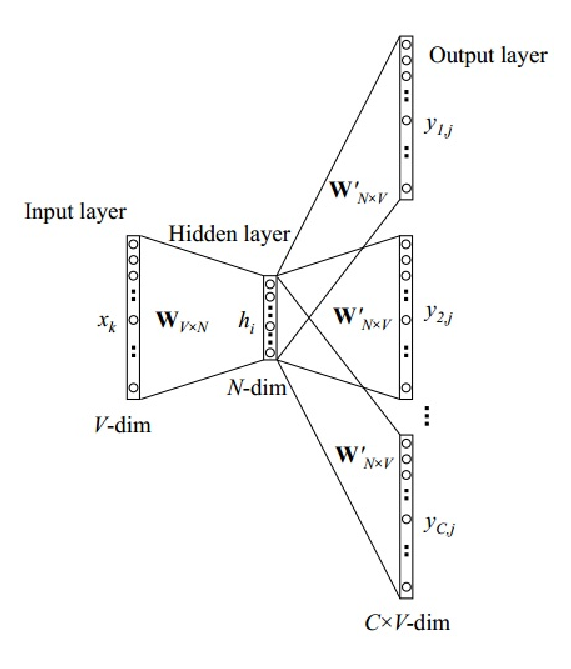
\includegraphics[width=90mm, height=90mm]{skipgram.eps}
\caption{Skip Gram Model(Figure from Rong (2014)) \label{fig:skipgram}}
\end{figure}
The main advantage of using skip-gram is that it is computationally less expensive than other neural language models with a complexity of O(log V) instead of O(V). They use hierarchical softmax~\cite{Morin:05} to achieve such computational efficiency.

\subsection{tf-idf}
\label{subsec:tfidf}
Let $D=d_1, d_2, d_3....d_N$ be $N$ documents under study and $T=t_1, t_2, t_3,....t_M$ be the $M$ unique terms in these documents, then each document can be represented as a $M$-dimensional vector:\\
$t_d=\{tf_1,tf_2,tf_3,...tf_M\}$\\
$tf-idf$ weights discounts the frequency of terms based on their importance to a particular document in the entire document set collection under consideration. This is done as follows:
\begin{center}
$tfidf(d,t)=tf(d,t) \times \log(\frac{|D|}{df(t)})$ 
\end{center}
Here $df(t)$ is the number of documents in which term $t$ appears.

\subsection{Vector Averaging for phrases}
\label{sec:vectoraveraging}
We will describe the process for Hindi but the same flow was followed for English as well.
As an output of the word vector learning, we now have a $n$-dimensional
vector representation for each word in the Hindi corpus.  Now we need to
assign features for sentences and paragraphs taken from the sentiment dataset
(training and test).  Mikolov et al. (2013b) and Levy et al. (2014) show that
many relational similarities can be recovered by means of vector arithmetic
in the embedded space.  Thus, additive models are useful, though
others have claimed that multiplicative models correlate better with human
judgments~\cite{Mitchell:08,Socher:13}.  In this work, we have retained the
simplicity of vector averaging to model larger chunks of  discourse.
This models the sentence/document in the same high dimensional space.

A preprocessing step involved removing some words that appear at very high or
very low frequencies in the corpus.  
Our model was trained on the Hindi Wikipedia dump to create vector
representations for words. The previous two vectors were concatenated to
create another feature set for training purpose.  
%?? SIZE of wikipedia corpus, number of independent words etc. 

\underline{\emph{Algorithm}}
\begin{enumerate}
%\setlength{\itemsep}{0.5pt}
\item Input the Hindi text corpus
\item Train skip-gram model to obtain word vector representation
\item Given a sentiment training set, obtain average vector data for each sentence/document
\item Obtain tf-idf vector for each sentence/document in the corpus
\item Concatenate vectors of step 3 and step 4 to obtain a feature set for a training instance
\item Train linear SVM with $m$-fold cross validation to create a classifier
(here $m$=20)
\end{enumerate}

\section{Document Vectors}
This distributed representation of sentences and documents~\cite{Le:14} modifies word2vec (Skip-Gram) algorithm to unsupervised learning of continuous representations for larger blocks of text, such as sentences, paragraphs or entire documents. The algorithm represents each document by a dense vector which is later trained and tuned to predict words in the sentence\/document.\\
In Paragraph Vector framework, every paragraph is mapped to a unique vector and id, represented by a matrix $D$, which is a column matrix. Every word is mapped to a unique vector and word vectors are concatenated or averaged to predict the context, i.e., the next word.\\
The change in this framework is that the $h$(in Skip-Gram model's equation) is now constructed in a different way. It is now constructed using both $W$ and $D$.\\
The contexts are fixed-length and sampled from a sliding window over the paragraph. The paragraph vector is shared across all contexts generated from the same paragraph but not across paragraphs.  The word vector matrix W, however, is shared across paragraphs. i.e., the vector for "good" is the same for all paragraphs.\\

The paragraph vectors and word vectors are trained using stochastic gradient descent and the gradient is obtained via backpropagation.  At every step of stochastic gradient descent, one can sample a fixed-length context from a random paragraph, compute the error gradient from the network in Figure \ref{fig:doc2vec} and use the gradient to update the parameters in our model. At prediction time, one needs to perform an inference step to compute the paragraph vector for a new paragraph. This is also obtained by gradient descent.  In this step, the parameters for the rest of the model, the word vectors W
and the softmax weights, are fixed.

\begin{figure}[ht!]
\centering
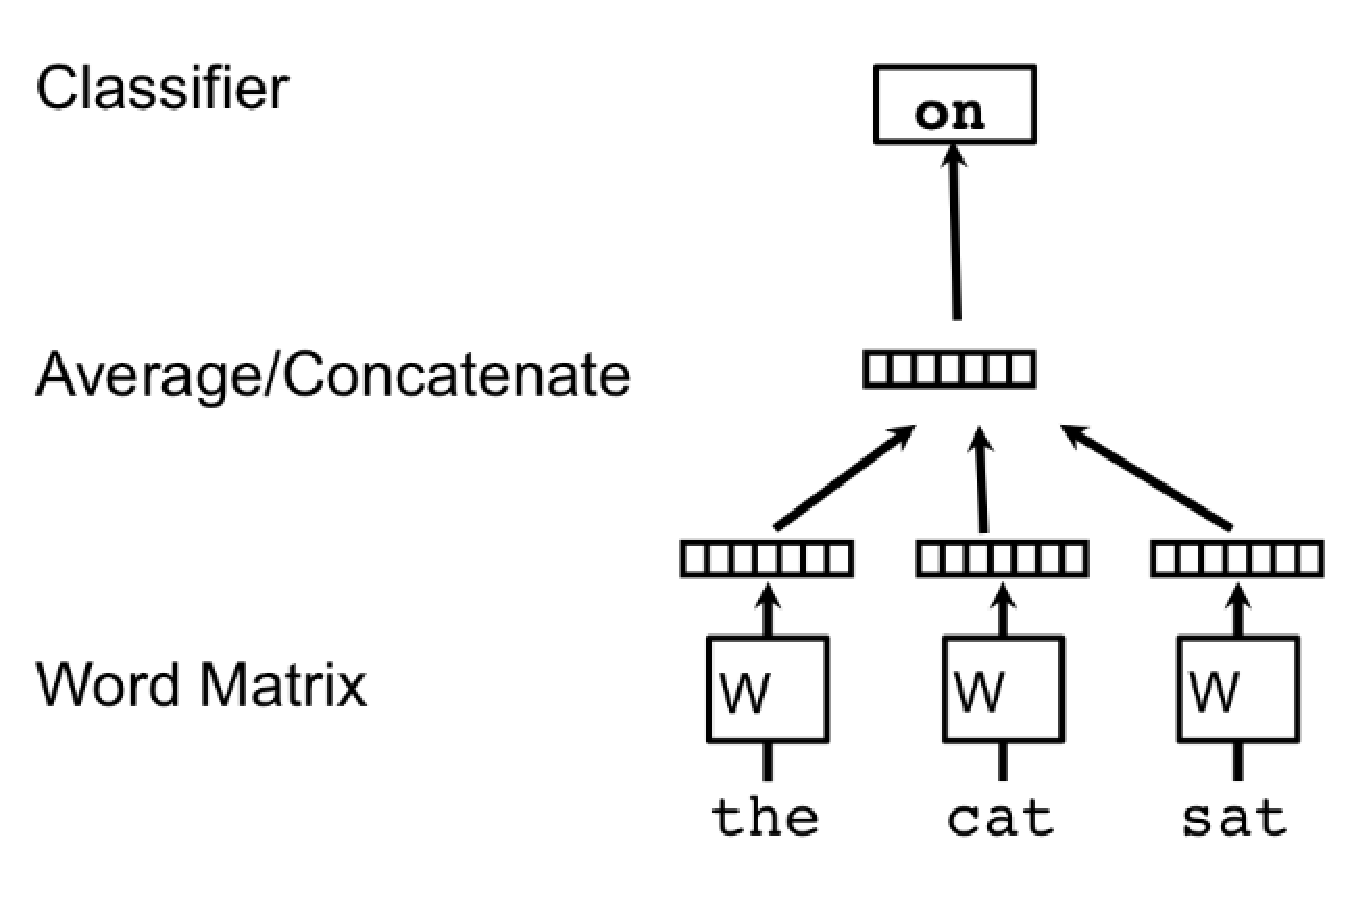
\includegraphics[width=110mm, height=70mm]{doc2vec_word_vector.eps}
\caption{Framework for learning word vectors(Figure from Le (2014)). \label{fig:word2vec}}
\end{figure}
In Figure \ref{fig:word2vec}, context  of three words ("the", "cat" and "sat") is used to predict the fourth word ("on"). The input words are mapped to columns of the matrix $W$ to predict the output word(Figure from Le (2014)).

\begin{figure}[ht!]
\centering
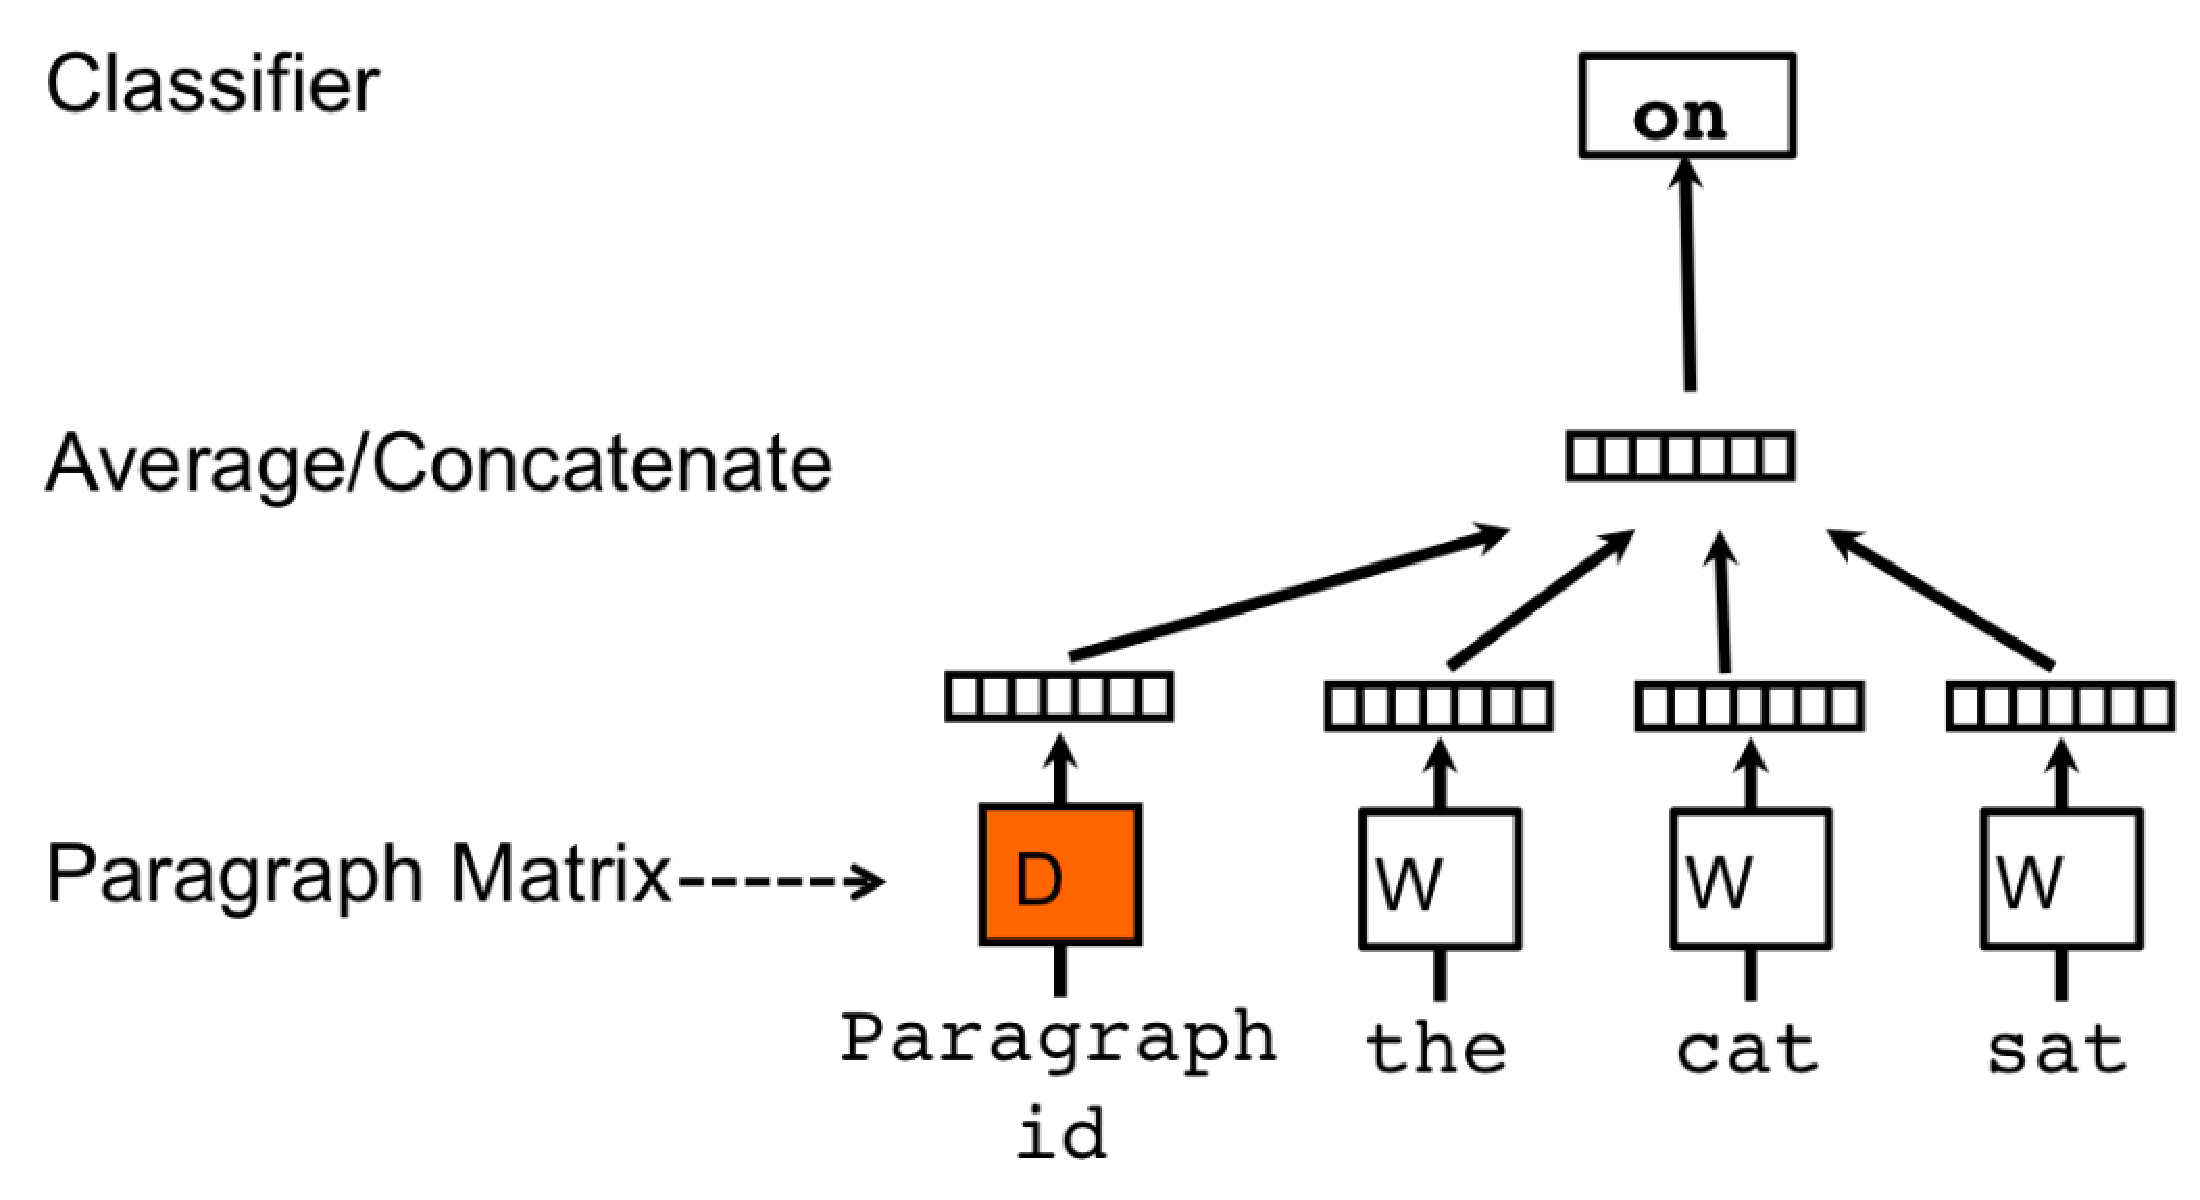
\includegraphics[width=110mm, height=70mm]{doc2vec.eps}
\caption{Framework for learning paragraph vectors(Figure from Le (2014)). \label{fig:doc2vec}}
\end{figure}
In Figure \ref{fig:doc2vec}, the only change is the additional paragraph token that is mapped to a vector via matrix $D$. In this model, the concatenation or average of this vector with a context of three words is used to predict the fourth word. The paragraph vector represents the missing information from the current context and can act as a memory of the topic of the paragraph.

The advantage of using paragraph vectors is that they inherit the property of word vectors, i.e., the semantics of the words. In addition, they also take into consideration a small context around each word which is in close resemblance to the n-gram model with a large n. This property is crucial because the n-gram model preserves a lot of information of the sentence/paragraph, which includes the word order also. This model also performs better than the Bag-of-Words model which would create a very high-dimensional representation that has very poor generalization.

\section{Recurrent Neural Network}
\label{sec:rnn}
The primary feature of a Recurrent Network is that it contains atleast one feed-back connection which captures dynamic temporal behavior and allows it to learn sequences. They have application in tasks such as prediction of a word given the context, perform sequence recognition/reproduction.\\
Recurrent Neural Networks have many different forms. One of them is a Fully Recurrent Network, a network of neuron-like units, each with a directed connection to every other unit.\\
\begin{figure}[ht!]
\centering
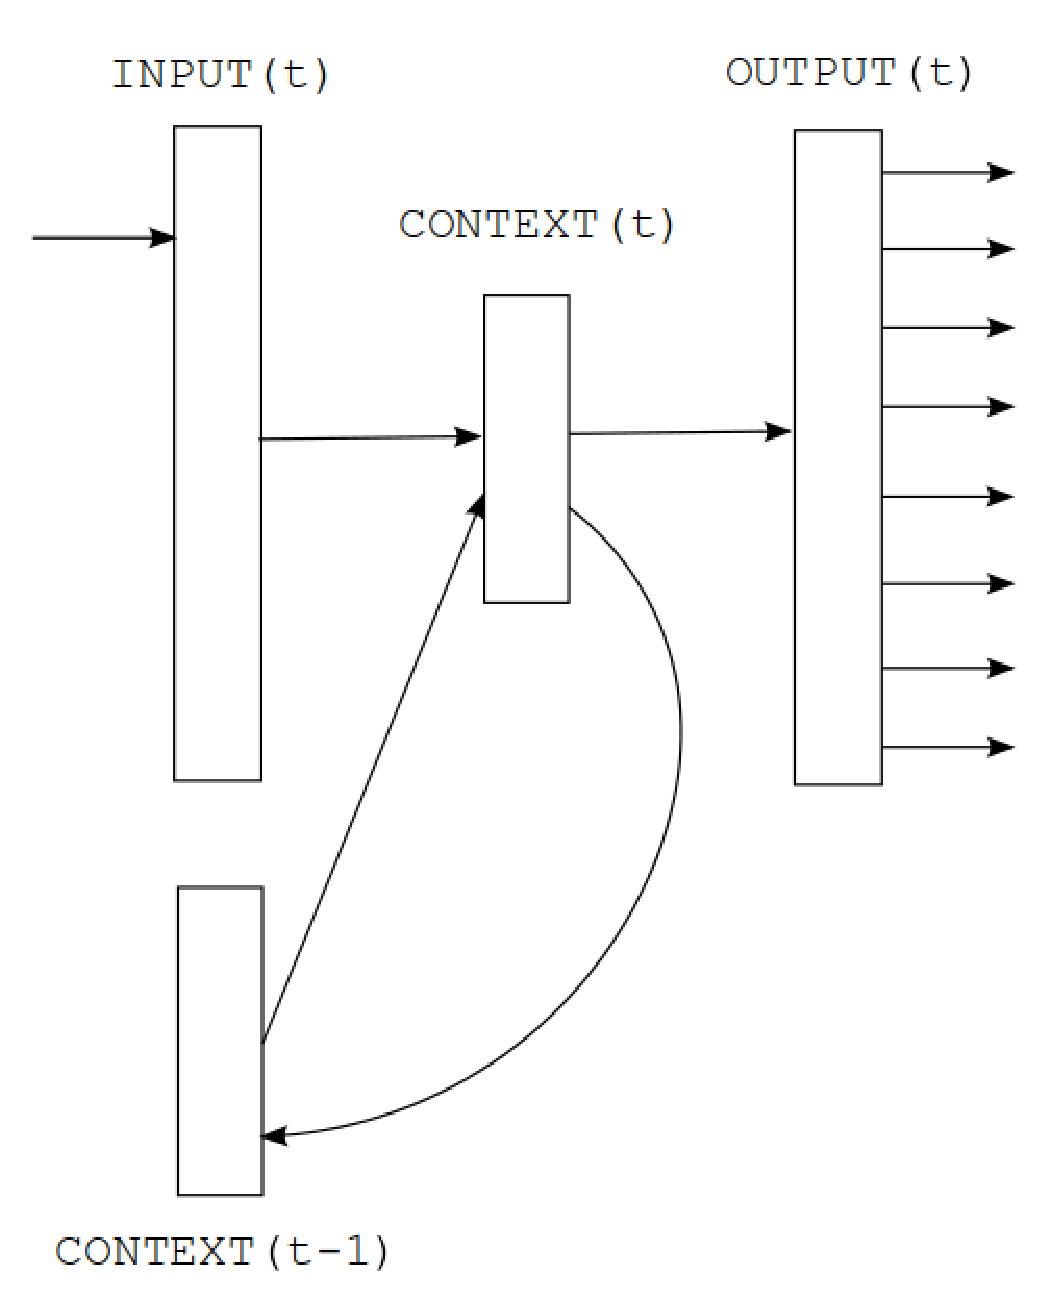
\includegraphics[width=70mm, height=70mm]{rnn.eps}
\caption{Simple Recurrent Neural Network(Figure from \cite{Mikolov:10}). \label{fig:rnn}}
\end{figure}

The architecture of a simple RNN consists of an input layer $x$, a hidden layer $s$(also known as context layer or network state) and an output layer $y$. Since the training is time dependent, we will denote input $x$ as $x(t)$, output $y$ as $y(t)$ and state $s$ as $s(t)$. Input vector $x(t)$ is a concatenation of vector $w$ representing current word, and output from neurons in context layer $s$ at time $t-1$(We can also include output from context layer before $t-1$ as well). The equations of each layer are described below:
\begin{align}
x(t) = w(t) + s(t-1) \\
s_j(t) = f\bigg(\sum_{i}x_i(t)u_{ji}\bigg) \\
y_k(t) = g\bigg(\sum_{j}s_j(t)v_{kj}\bigg)
\end{align}
where $f(z)$ is sigmoid function for activation and $g(z)$ is a softmax function for output prediction:
\begin{align}
f(z) = \frac{1}{1+\mathrm{e}^{-z}} \\
g(z_m) = \frac{\mathrm{e}^{z_m}}{\sum_{k}\mathrm{e}^{z_k}}
\end{align}

\cite{Mikolov:10} claim that size of hidden layer reflects amount of training data with smaller size leading to less number of layers. Weights are initialized to random small values and updated using gradient descent. Output layer $y(t)$ represents probability distribution of next word given previous word $w(t)$ and context $s(t-1)$. The objective function is:
\begin{align}
error(t) =  actual(t) - y(t)
\end{align}
where $actual(t)$ is a $1$-hot vector representing the word that should have been predicted given the context.
\begin {table}[h!]
\centering
\begin{tabular}{ |c|c|c| }
\hline
Model & DEV WER & EVAL WER \\ \hline
Lattice 1 best & 12.9 & 18.4 \\ 
Baseline-KN5 (37M) & 12.2 & 17.2 \\
Discriminative LM (37M) & 11.5 & 16.9 \\
Joint LM (70M) (37M) & - & 16.7 \\ \hline
Static 3xRNN + KN5 (37M) & 11.0 & 15.5 \\
Dynamic 3xRNN + KN5 (37M) & 10.7 & 16.3 \\
\hline
\end{tabular}
\caption {Comparison of WSJ results obtained with various models(RNN is trained on just 6.4M words)}
\label{table:rnn}
\end{table}
Table \ref{table:rnn} represents results of \cite{Mikolov:10} obtained in WSJ experiments using RNN.\\

\cite{Mikolov:11} present several modifications of the original recurrent neural network language model (RNN LM). The present approaches that lead to more than 15 times speedup for both training and testing phases. They also show the importance of backpropagation through time(BPTT) which is an extension to backpropagation algorithm for recurrent networks. With truncated BPTT, the error is propagated through recurrent connections back in time for a specific number of time steps. Thus, the network learns to remember information for several time steps in the hidden layer when it is learned by the BPTT.\\
The speedup is obtained by assuming that words can be mapped to classes. Thus if we assume that each word belongs to exactly one class, we can first estimate the probability distribution over each class using RNN and then calculate the probability of a particular word from the desired class assuming unigram distribution of words within the class. Thus, now we are reducing the connections between hidden and output layer from $V$ to $C$ which is a significant improvement.\\
They are often very sensitive to small changes in its parameters which changes the gradient by a large amount. Few others are, Bi-directional RNN and Hierarchical RNN.\\

\section{Semantic Composition}
\label{sec:composition}
The Principle of Compositionality is that meaning of a complex expression is determined by the meaning of its parts or constituents and the rules which guide this combination. It is also known as \emph{Frege's Principle}. In our case, the constituents are word vectors and the expression in hand is the sentence/document vector. For example,
\begin{center}
\emph{The movie is funny and the screenplay is good}
\end{center}
In the above sentence, consider the word vectors are represented by $w(x)$ and the sentence vector as $S(x)$. Hence,
\begin{align}
S(x) = c_1w_1(x) \Theta c_2w_2(x) \Theta c_3w_3(x) \Theta c_4w_4(x) \dots \Theta c_kw_k(x)
\end{align}
where $\Theta$ can be any operation(e.g., addition, multiplication) and $c_i$s are constants.

\begin {table}[h!]
\centering
\begin{tabular}{ |c|c| }
\hline
Composition & Accuracy \\ \hline \hline
Average & 88.42 \\ \hline
Weighted Average & 88.41 \\ \hline
Multiplication & 50.30 \\ \hline
\end{tabular}
\caption {Results of Vector Composition with different Operations}
\label{table:composition}
\end{table}
Analyzing the results from Table \ref{table:composition}, we observed that when we deal with large number of features, there is a presence of large number of \emph{zeros} and presence of a single zero in a feature will make that features contribution zero in the final vector, which happens in our case and thus multiplicative composition fails.\\
We, therefore, adopt both simple and weighted average methods in our work. The advantage with addition is that, it doesnot increase the dimension of the vector and captures high level semantics with ease. In fact, \cite{Zou:13} have used simple average to construct phrase vectors which they have later used to find phrase level similarity using cosine distance.\\
\cite{Mikolov:13c} showed that relations between words are reflected to a large extent in the offsets between their vector embeddings. They also use additive composition to reflect semantic dependencies.
\begin{center}
\emph{queen - king $\approx$ woman - man}
\end{center}
\cite{Blacoe:12} clearly show that vectors of Neural Language Model and Distributed Model when used with additive composition outperform those with multiplicative composition in Paraphrase Classification task. DM vectors outperform by nearly giving accuracy difference of 6\%. They also perform very well on Phrase similarity tasks.\\
\cite{Socher:13} also present yet another model for semantic composition but that uses a sentiment treebank which is a very costly structure to build and it is task dependent. For under-resourced languages such as Hindi, it would take years to build (for English, task done through Amazon Mechanical Turk). This leads to appreciation of models such as Additive Composition.\\
\begin{figure}[H]
\centering
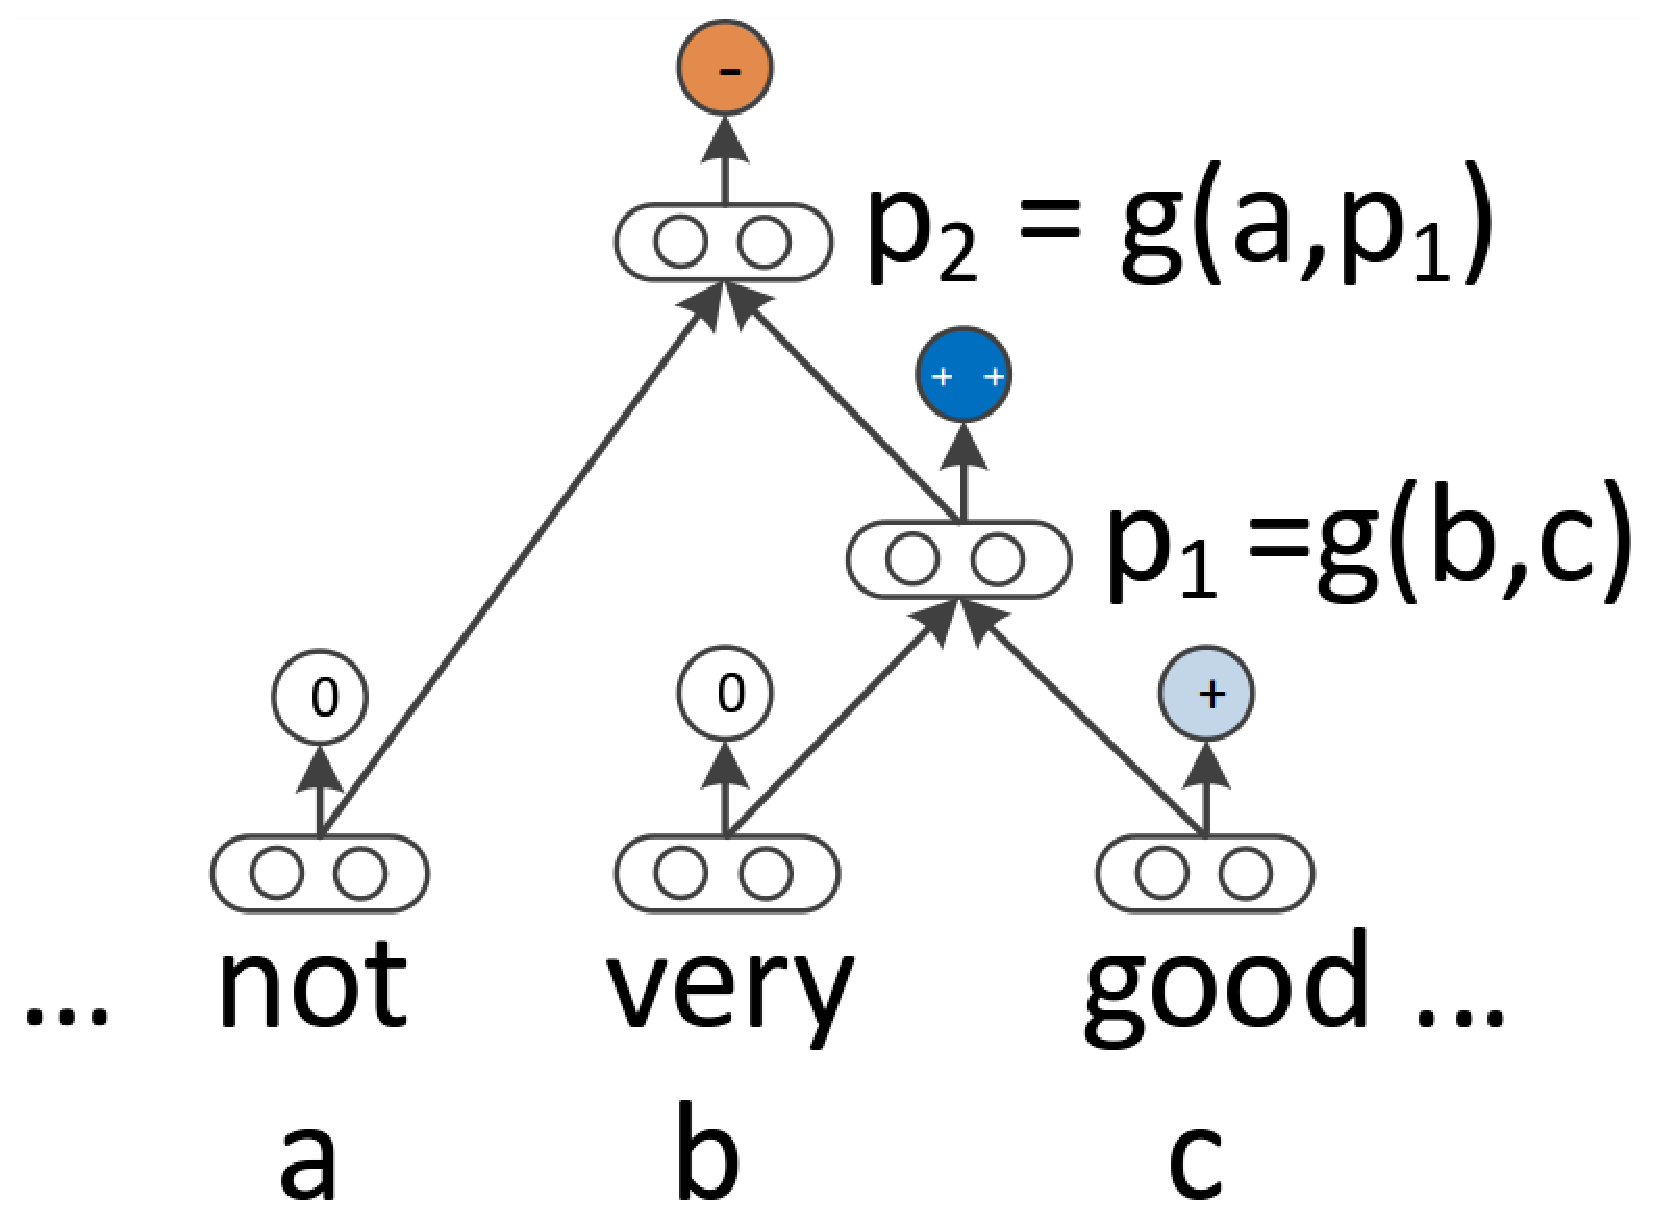
\includegraphics[width=90mm, height=80mm]{recursiveNN.eps}
\caption{Approach of Recursive Neural Network(Figure from \cite{Socher:13}). \label{fig:recursiveNN}}
\end{figure}
Figure \ref{fig:recursiveNN} depicts the approach of recursive neural network. When an n-gram is given to the compositional models, it is parsed into a binary tree and each leaf node, corresponding to a word, is represented as a vector. Recursive neural models will then  compute parent vectors in a bottom up fashion using different types of compositionality functions $g$. The parent vectors are again given as features to a classifier.


	\chapter{Background}
	The algorithms and data structures used in this thesis have been introduced and discussed below.
	\section{Word-Vectors by using Skip-Gram}
	\label{sec:skipgram}
Mikolov et al. (2013b) proposed two neural network models for building word vectors from large unlabelled corpora; Continuous Bag of Words(CBOW) and Skip-Gram.  In the CBOW model, the context is the input, and one tries to learn a vector for the central word; in Skip grams, the input is the target word and one tries to guess the set of contexts.  The Skip gram was found to perform better on smaller corpora, and here we have focused on this model for building our word vectors. The model uses each current word as an input to a log-linear classifier with continuous projection layer, and predict words within a certain range before and after the current word. The objective is to maximize the probability of the context given a word within a language model:

\begin{center} $p(c|w;\theta)=\frac{\exp^{v_c.v_w}}{\sum_{c' \in C}\exp^{v_c.v_w}}$ \end{center}
where $v_c$ and $v_w$ $\in$ $R^d$ are vector representations for context $c$ and word $w$ respectively. $C$ is the set of all available contexts. The parameters $\theta$ are $v_ci$, $v_wi$ for $w \in V$, $c \in C$, $i \in 1,....,d$ (a total of $|C| \times |V| \times d$ parameters).\\

The weights between the input layer and the output layer can be represented by a $V \times N$ matrix \textbf{W}. Each row of \textbf{W} is the $N$-dimension vector representation $v_w$ of the associated word of the input layer.Given a word, assuming $x_k=1$ and $x_{k'}=0$ for $k' \neq k$, then
\begin{center}
$h=x^TW=W_{(k,.)}:=v_{w_I}$
\end{center}
which is essentially copying the $k$-th row of \textbf{W} to \textbf{h}. $v_{w_I}$ is the vector representation of the input word $w_I$.

From the hidden layer to the output layer, there is a different weight matrix \textbf{W'}=$\{w_{ij}^{'}\}$ which is a $N \times V$ matrix. Then we can use soft-max, a log-linear classification model, to obtain the posterior distribution of words, which is a multinomial distribution.\\
On the output layer, instead of outputing one multinomial distribution, we are outputing C multinomial distributions. Each output is computed using the same hidden$\rightarrow$output matrix.
\begin{center}
$p(w_{c,j}=w_{O,c}|w_I)=y_{c,j}=\frac{exp(u_{c,j})}{\sum_{j'=1}^{V}exp(u_{j'})}$
\end{center}
where $w_{c,j}$ is the $j$-th word on the $c$-th panel of the output layer; $w_{O,c}$ is the actual $c$-th word in the output context words; $w_I$ is the only input word; $y_{c,j}$ is the output of the $j$-th node on the $c$-th panel of the output layer; $u_{c,j}$ is the net input of the $j$-th node on the $c$-th panel of the output layer.
Because the output layer panels share the same weights, thus
\begin{center}
$u_{c,j}=u_j=v`_{w_j}^T.h$, for $c=1,2...,C$
\end{center}
where $v'_{w_j}$ is the output vector of the $j$-th word in the vocabulary, $w_j$, and also $v'_{w_j}$ is taken from a column of the hidden$\rightarrow$output weight matrix, \textbf{W'} .

The loss function is
\begin{center}
E = -$\log p(w_{O,1},w_{O,2},....,w_{O,C}|w_I)$\\
=-$\log \prod_{c=1}^{C}\frac{exp(u_{c,j_{c}^{*	}})}{\sum_{j'=1}^{V}exp(u_{j'})}$\\
=-$\sum_{c=1}^{C} u_{j_{c}^{*}}+C.\log \sum_{j'=1}^{V}exp(u_{j'})$
\end{center}
where $j_{c}^{*}$ is the index of the actual $c$-th output context word in the vocabulary.

After taking the necessary derivatives, the update equation for the hidden$\rightarrow$output weight matrix, \textbf{W'},
\begin{center}
$w'{ij}^{(new)}=w'{ij}^{(old)}-\eta .EI_j.h_i$
\end{center}
or,
\begin{center}
$v'{w_j}^{(new)}=v'{w_j}^{(old)}-\eta .EI_j.\textbf{h}$ for $j=1,2,.....,V$
\end{center}

The update equation for the input$\rightarrow$hidden weight matrix, \textbf{W},
\begin{center}
$v{w_I}^{(new)}=v{w_I}^{(old)}-\eta .EH$
\end{center}
where $EH$ is a $N$-dimensional vector. Its each component is defined as
\begin{center}
$EH_i=\sum_{j=1}^{V}EI_j.w'_{ij}$
\end{center}

\begin{figure}[ht!]
\centering
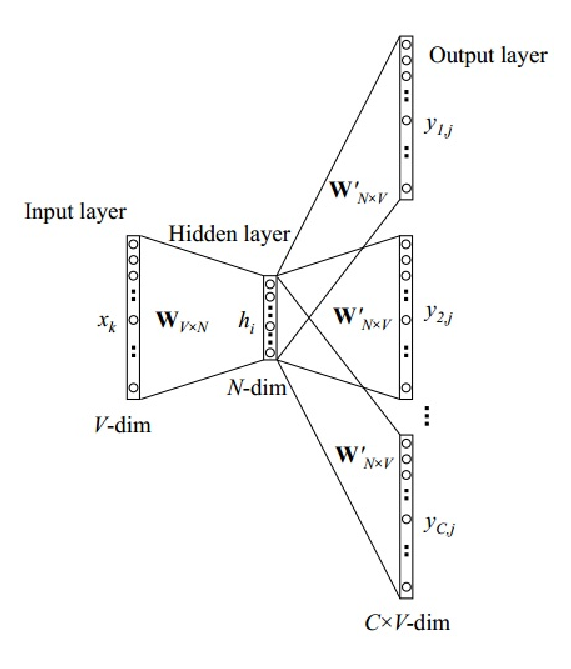
\includegraphics[width=70mm, height=70mm]{skipgram.eps}
\caption{Skip Gram Model(Figure from Rong (2014)) \label{fig:skipgram}}
\end{figure}

\subsection{tf-idf}
\label{subsec:tfidf}
Let $D=d_1, d_2, d_3....d_N$ be $N$ documents under study and $T=t_1, t_2, t_3,....t_M$ be the $M$ unique terms in these documents, then each document can be represented as a $M$-dimensional vector:\\
$t_d=\{tf_1,tf_2,tf_3,...tf_M\}$\\
$tf-idf$ weights discounts the frequency of terms based on their importance to a particular document in the entire document set collection under consideration. This is done as follows:
\begin{center}
$tfidf(d,t)=tf(d,t) \times \log(\frac{|D|}{df(t)})$ 
\end{center}
Here $df(t)$ is the number of documents in which term $t$ appears.

\subsection{Vector Averaging for phrases}
	\label{sec:vectoraveraging}
As an output of the word vector learning, we now have a $n$-dimensional
vector representation for each word in the Hindi corpus.  Now we need to
assign features for sentences and paragraphs taken from the sentiment dataset
(training and test).  Mikolov et al. (2013b) and Levy et al. (2014) show that
many relational similarities can be recovered by means of vector arithmetic
in the embedded space.  Thus, additive models are useful, though
others have claimed that multiplicative models correlate better with human
judgments~\cite{Mitchell:08,Socher:13}.  In this work, we have retained teh
simplicity of vector averaging to model larger chunks of  discourse.
This models the sentence/document in the same high dimensional space.

A preprocessing step involved removing some words that appear at very high or
very low frequencies in the corpus.  
Our model was trained on the Hindi Wikipedia dump to create vector
representations for words. The previous two vectors were concatenated to
create another feature set for training purpose.  
%?? SIZE of wikipedia corpus, number of independent words etc. 

\underline{\emph{Algorithm}}
\begin{enumerate}
%\setlength{\itemsep}{0.5pt}
\item Input the Hindi text corpus
\item Train skip-gram model to obtain word vector representation
\item Given a sentiment training set, obtain average vector data for each sentence/document
\item Obtain tf-idf vector for each sentence/document in the corpus
\item Concatenate vectors of step 3 and step 4 to obtain a feature set for a training instance
\item Train linear SVM with $m$-fold cross validation to create a classifier
(here $m$=20)
\end{enumerate}

\section{Document Vectors}
This distributed representation of sentences and documents~\cite{Le:14} modifies wors2vec (Skip-Gram) algorithm to unsupervised learning of continuous representations for larger blocks of text, such as sentences, paragraphs or entire documents. The algorithm represents each document by a dense vector which is later trained and tuned to predict words in the sentence\/document.\\
In Paragraph Vector framework, every paragraph is mapped to a unique vector and id, represented by a matrix $D$, which is a column matrix. Every word is mapped to a unique vector and word vectors are conactenated or averaged to predict the context, i.e., the next word.\\
The change in this framework is that the $h$(in Skip-Gram model's equation) is now constructed in a different way. It is now constructed using both $W$ and $D$.\\
The contexts are fixed-length and sampled from a sliding window over the paragraph. The paragraph vector is shared across all contexts generated from the same paragraph but not across paragraphs.  The word vector matrix W, however, is shared across paragraphs. i.e., the vector for "good" is the same for all paragraphs.\\

The paragraph vectors and word vectors are trained using stochastic gradient descent and the gradient is obtained via backpropagation.  At every step of stochastic gradient descent, one can sample a fixed-length context from a random paragraph, compute the error gradient from the network in Figure \ref{fig:doc2vec} and use the gradient to update the parameters in our model. At prediction time, one needs to perform an inference step to compute the paragraph vector for a new paragraph. This is also obtained by gradient descent.  In this step, the parameters for the rest of the model, the word vectors W
and the softmax weights, are fixed.

\begin{figure}[ht!]
\centering
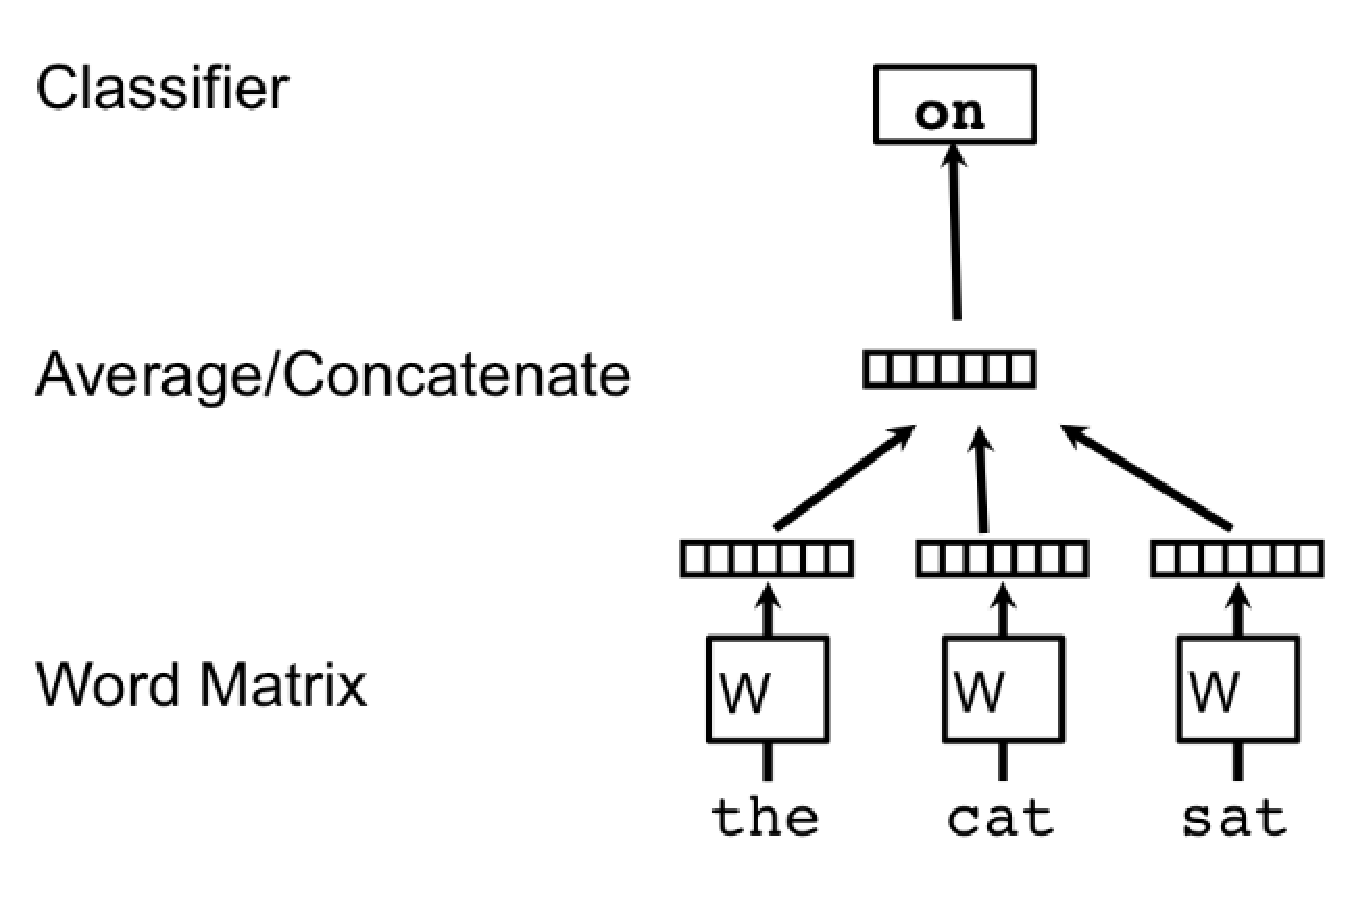
\includegraphics[width=110mm, height=70mm]{doc2vec_word_vector.eps}
\caption{Framework for learning word vectors(Figure from Le (2014)). \label{fig:word2vec}}
\end{figure}
In Figure \ref{fig:word2vec}, context  of three words ("the", "cat" and "sat") is used to predict the fourth word ("on"). The input words are mapped to columns of the matrix $W$ to predict the output word(Figure from Le (2014)).

\begin{figure}[ht!]
\centering
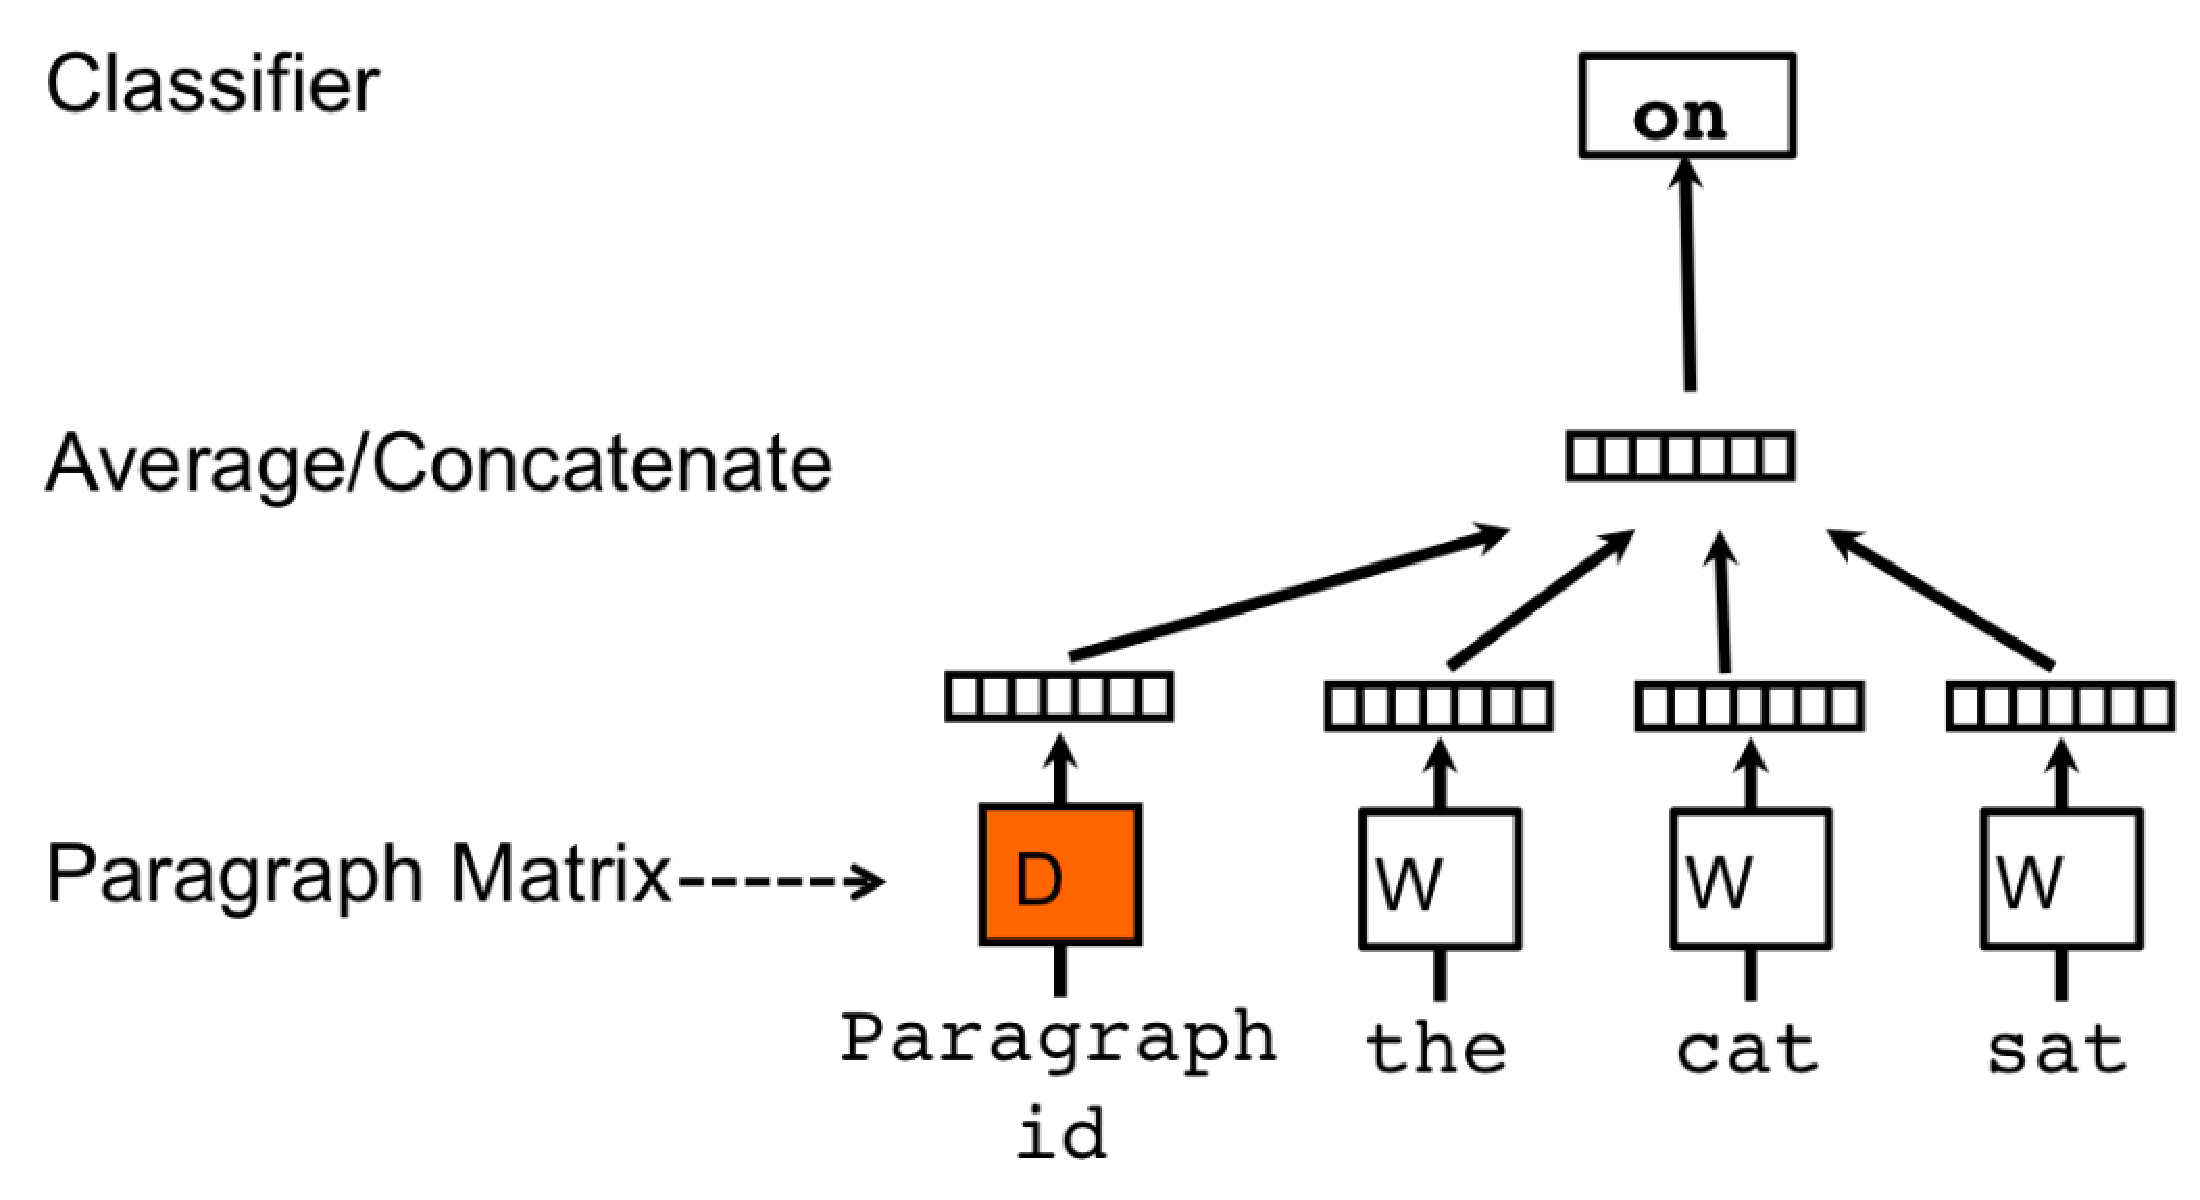
\includegraphics[width=110mm, height=70mm]{doc2vec.eps}
\caption{Framework for learning paragraph vectors(Figure from Le (2014)). \label{fig:doc2vec}}
\end{figure}
In Figure \ref{fig:doc2vec}, the only change is the additional paragraph token that is mapped to a vector via matrix $D$. In this model, the concatenation or average of this vector with a context of three words is used to predict the fourth word. The paragraph vector represents the missing information from the current context and can act as a memory of the topic of the paragraph.

The advantage of using paragraph vectors is that they inherit the propery of word vectors, i.e., the semantics of the words. In addition, they also take into consideration a small context around each word which is in close resemblance to the n-gram model with a large n. This property is crucial because the n-gram model preserves a lot of information of the sentence\/paragraph, which includes the word order also. This model also performs better than the Bag-of-Words model which would create a very high-dimensional representation that has very poor generalization.

\section{Recurrent Neural Network}
\label{sec:rnn}
The primary feature of a Recurrent Network is that it contains atleast one feed-back connection which captures dynamic temporal behavior and allows it to learn sequences. They have application in tasks such as prediction of a word given the context, perform sequence recognition/reproduction.\\
Recurrent Neural Networks have many different forms. One of them is a Fully Recurrent Network, a network of neuron-like units, each with a directed connection to every other unit.\\
\begin{figure}[ht!]
\centering
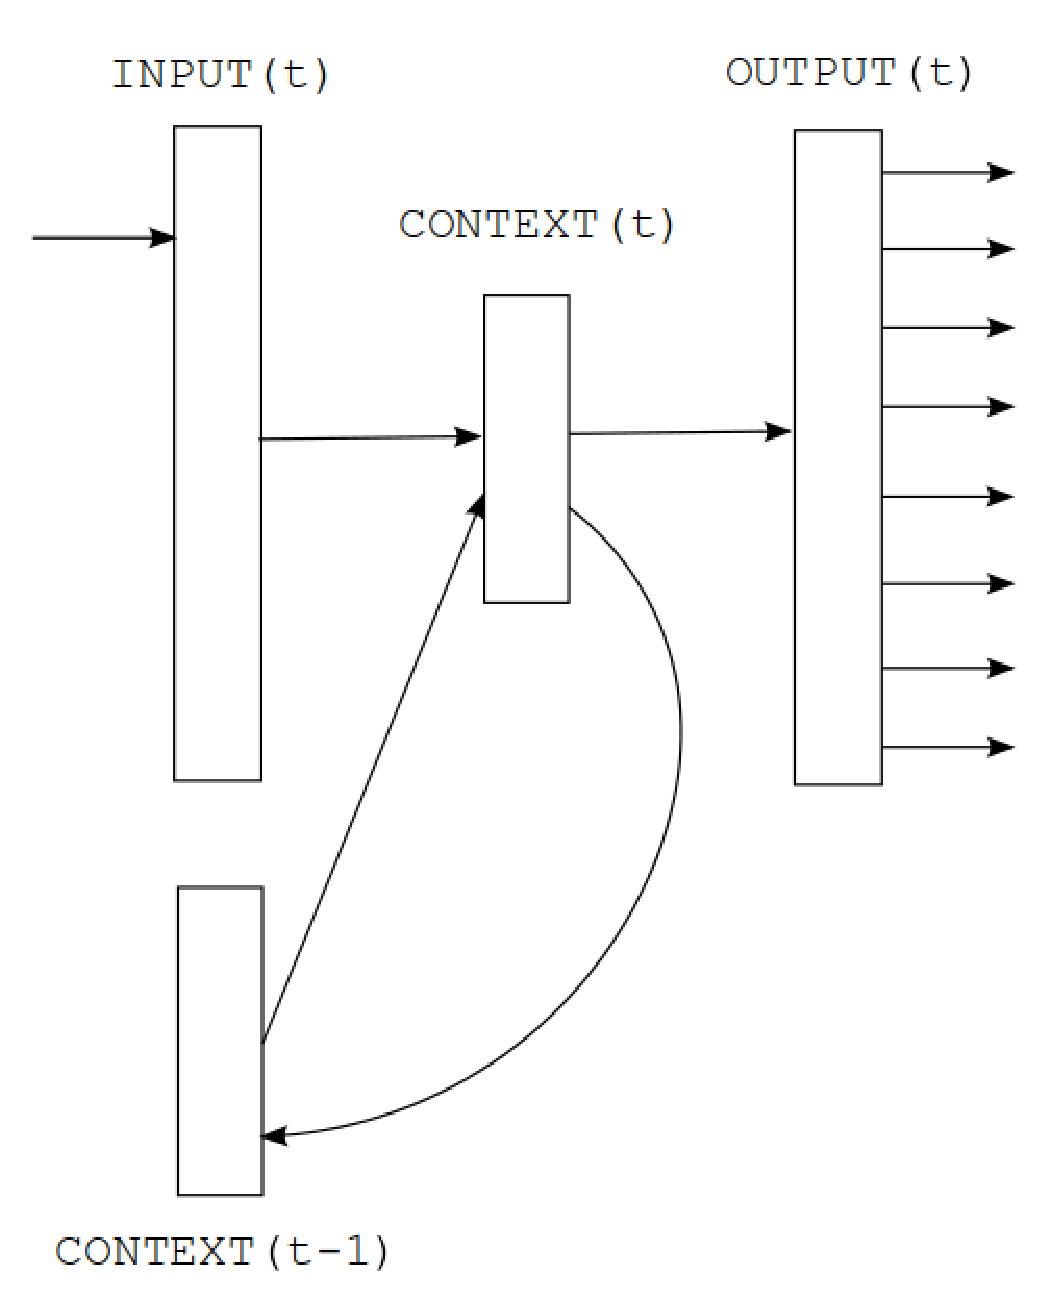
\includegraphics[width=70mm, height=70mm]{rnn.eps}
\caption{Simple Recurrent Neural Network(Figure from \cite{Mikolov:10}). \label{fig:rnn}}
\end{figure}

The architecture of a simple RNN consists of an input layer $x$, a hidden layer $s$(also known as context layer or network state) and an output layer $y$. Since the training is time dependent, we will denote input $x$ as $x(t)$, output $y$ as $y(t)$ and state $s$ as $s(t)$. Input vector $x(t)$ is a concatentaion of vector $w$ representing current word, and output from neurons in context layer $s$ at time $t-1$(We can also include output from context layer before $t-1$ as well). The equations of each layer are described below:
\begin{align}
x(t) = w(t) + s(t-1) \\
s_j(t) = f\bigg(\sum_{i}x_i(t)u_{ji}\bigg) \\
y_k(t) = g\bigg(\sum_{j}s_j(t)v_{kj}\bigg)
\end{align}
where $f(z)$ is sigmoid function for activation and $g(z)$ is a softmax function for output prediction:
\begin{align}
f(z) = \frac{1}{1+\mathrm{e}^{-z}} \\
g(z_m) = \frac{\mathrm{e}^{z_m}}{\sum_{k}\mathrm{e}^{z_k}}
\end{align}

\cite{Mikolov:10} claim that size of hidden layer reflects amount of training data with smaller size leading to less number of layers. Weights are initialized to random small values and updated using gradient descent. Output layer $y(t)$ represents probability distribution of next word given previous word $w(t)$ and context $s(t-1)$. The objective function is:
\begin{align}
error(t) =  actual(t) - y(t)
\end{align}
where $actual(t)$ is a $1$-hot vector representing the word that should have been predicted given the context.
\begin {table}[h!]
\centering
\begin{tabular}{ |c|c|c| }
\hline
Model & DEV WER & EVAL WER \\ \hline
Lattice 1 best & 12.9 & 18.4 \\ 
Baseline-KN5 (37M) & 12.2 & 17.2 \\
Discriminative LM (37M) & 11.5 & 16.9 \\
Joint LM (70M) (37M) & - & 16.7 \\ \hline
Static 3xRNN + KN5 (37M) & 11.0 & 15.5 \\
Dynamic 3xRNN + KN5 (37M) & 10.7 & 16.3 \\
\hline
\end{tabular}
\caption {Comparison of WSJ results obtained with various models(RNN is trained on just 6.4M words)}
\label{table:rnn}
\end{table}
Table \ref{table:rnn} representes results of \cite{Mikolov:10} obtained in WSJ experiments using RNN.\\

\cite{Mikolov:11} present several modifications of the original recurrent neural network language model (RNN LM). The present approaches that lead to more than 15 times speedup for both training and testing phases. They also show the importance of backpropagation through time(BPTT) which is an extension to backpropagation algorithm for recurrent networks. With truncated BPTT, the error is propagated through recurrent connections back in time for a specific number of time steps. Thus, the network learns to remember information for several time steps in the hidden layer when it is learned by the BPTT.\\
The speedup is obtained by assuming that words can be mapped to classes. Thus if we assume thate ach word belongs to exactly one class, we can first estimate the probability distribution over each class using RNN and then calculate the probability of a particular word from the desired class assuming unigram distribution of words within the class. Thus, now we are reducing the connections between hidden and output layer from $V$ to $C$ which is a significant improvement.\\
They are often very sensitive to small changes in its parameters which changes the gradient by a large amount. Few others are, Bi-directional RNN and Hierarchical RNN.\\

\section{Semantic Composition}
\label{sec:composition}
The Principle of Compositionality is that meaning of a complex expression is determined by the meaning of its parts or constituents and the rules which guide this combination. It is also known as \emph{Frege's Principle}. In our case, the constituents are word vectors and the expression in hand is the sentence/document vector. For example,
\begin{center}
\emph{The movie is funny and the screenplay is good}
\end{center}
In the above sentence, consider the word vectors are represented by $w(x)$ and the sentence vector as $S(x)$. Hence,
\begin{align}
S(x) = c_1w_1(x) \Theta c_2w_2(x) \Theta c_3w_3(x) \Theta c_4w_4(x) \dots \Theta c_kw_k(x)
\end{align}
where $\Theta$ can be any operation(e.g., addition, multiplication) and $c_i$s are constants.

\begin {table}[h!]
\centering
\begin{tabular}{ |c|c| }
\hline
Composition & Accuracy \\ \hline \hline
Average & 88.42 \\ \hline
Weighted Average & 88.41 \\ \hline
Multiplication & 50.30 \\ \hline
\end{tabular}
\caption {Results of Vector Composition with different Operations}
\label{table:composition}
\end{table}
Analyzing the results from Table \ref{table:composition}, we observed that when we deal with large number of features, there is a presence of large number of \emph{zeros} and presence of a single zero in a feature will make that features contribution zero in the final vector, which happens in our case and thus multiplicative composition fails.\\
We, therefore, adopt both simple and weighted average methods in our work. The advantage with addition is that, it doesnot increase the dimensionof the vector and captures high level semantics with ease. In fact, \cite{Zou:13} have used simple average to construct phrase vectors which they have later used to find phrase level similarity using cosine distance.\\
\cite{Mikolov:13c} showed that relations between words are reflected to a large extent in the offsets between their vector embeddings. They also use additive composition to reflect semantic dependencies.
\begin{center}
\emph{queen - king $\approx$ woman - man}
\end{center}
\cite{Blacoe:12} clearly show that vectors of Neural Language Model and Distributed Model when used with additive composition outperform those with multiplicative composition in Paraphrase Classification task. DM vectors outperform by nearly giving accuracy difference of 6\%. They also perfrom very well on Phrase simliarity tasks.\\
\cite{Socher:13} also present yet another model for semantic composition but that uses a sentiment treebank which is a very costly structure to build and it is task dependent. For under-resourced languages such as Hindi, it would take years to build (for English, task done through Amazaon Mechanical Turk). This leads to appreciation of models such as Additive Composition.\\
\begin{figure}[ht!]
\centering
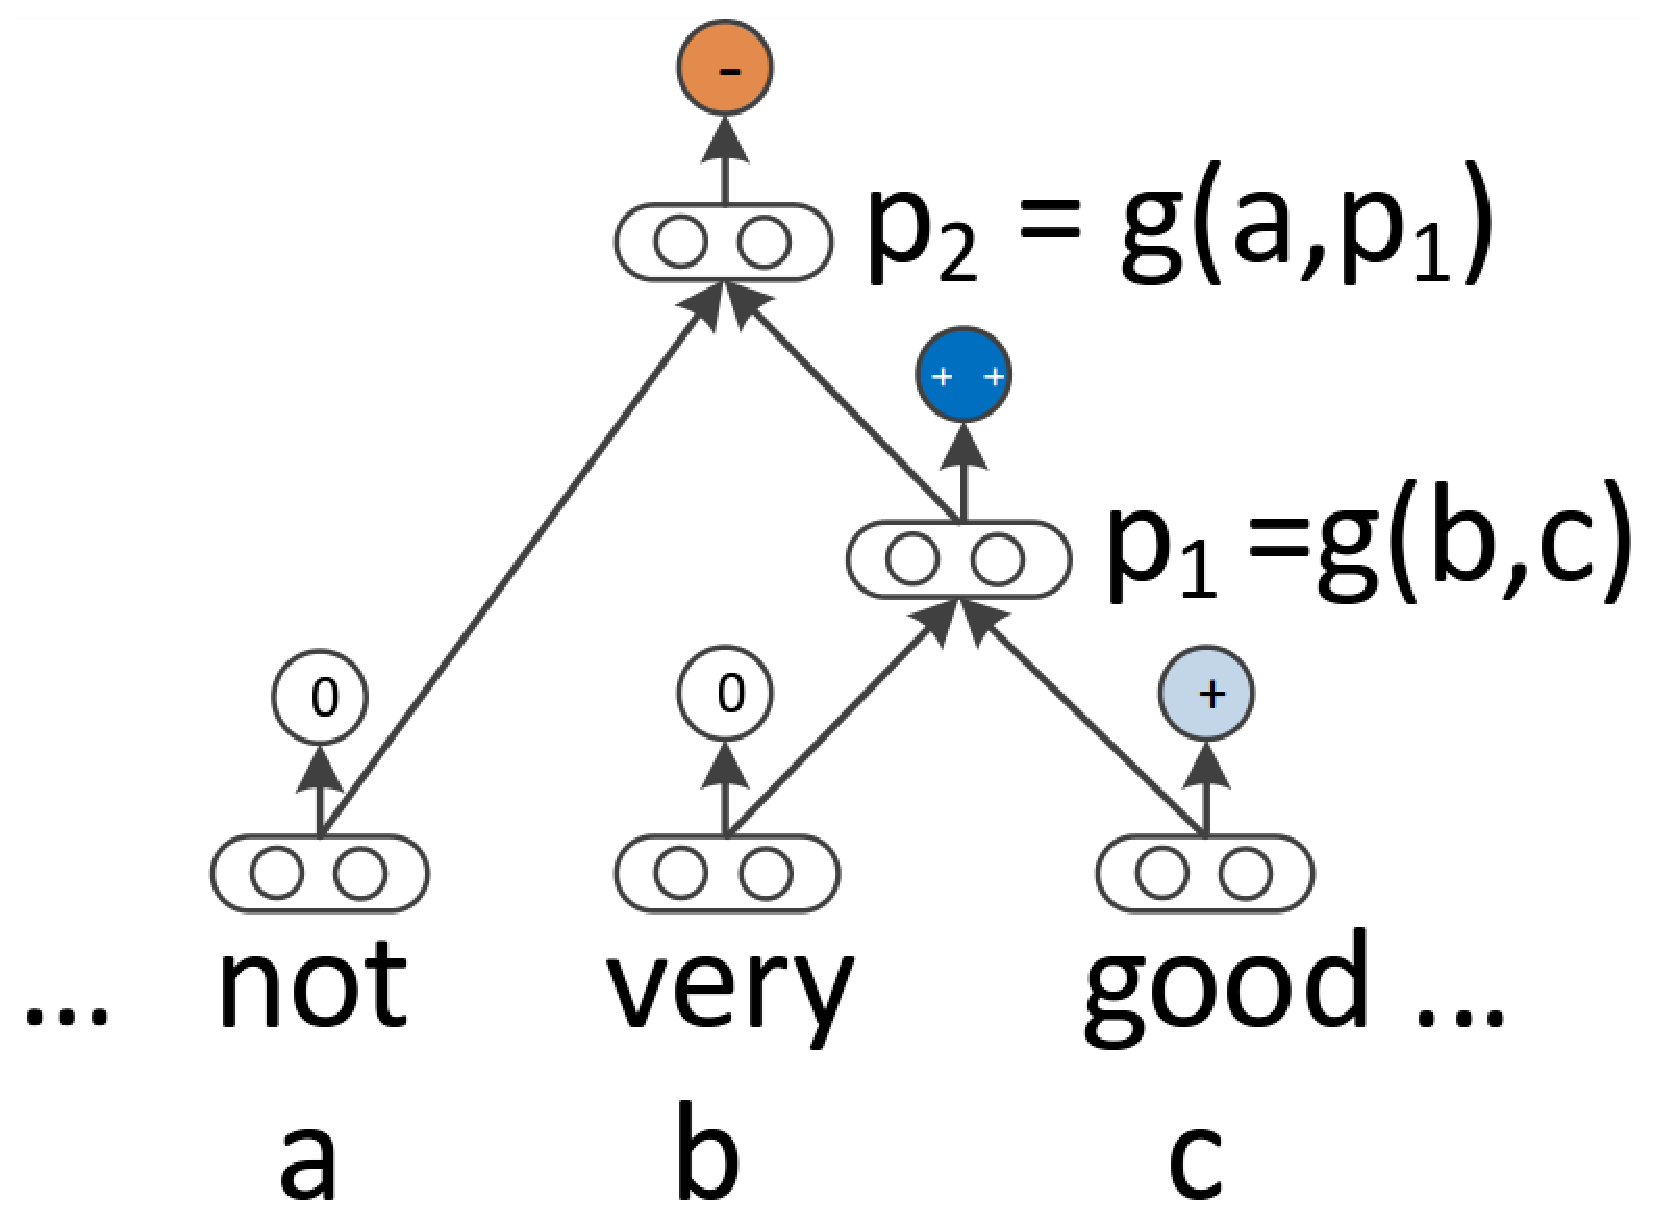
\includegraphics[width=90mm, height=80mm]{recursiveNN.eps}
\caption{Approach of Recursive Neural Network(Figure from \cite{Socher:13}). \label{fig:recursiveNN}}
\end{figure}
Figure \ref{fig:recursiveNN} depicts the approach of recursive neural network. When an n-gram is given to the compositional models, it is parsed into a binary tree and each leaf node, corresponding to a word, is represented as a vector. Recursive neural models will then  compute parent vectors in a bottom up fashion using different types of compositionality functions $g$. The parent vectors are again given as features to a classifier.


	\chapter{Data Acquisition}
\label{sec:data}
This section describes the corpus used in our experiments.

\section{Hindi Corpus}
\label{hindi_corpus}
\subsection{Product and Movie Review Corpus}
We experimented on two Hindi review datasets. One is the Product Review dataset (LTG, IIIT Hyderabad) containing 350 Positive reviews and 350 Negative reviews. The other is a Movie Review dataset (CFILT, IIT Bombay) containing 127 Positive reviews and 125 Negative reviews.\\
Each review is around 1-2 sentences long and the sentences are mainly focused on sentiment, either positive or negative.

\subsection{700-Movie Review Corpus(Our Contribution)}
\label{new_reviews}
We collected Hindi movie reviews from websites such as \emph{Dainik Jagran} and \emph{Navbharat Times}. The movie reviews are longer than the previous corpus and contains subjects other than sentiment.
There are in total 697 movie reviews from both the websites. The statistics compiled is described below.\\

\begin {table}[h!]
\large
\centering
\begin{tabular}{ |l|l| }
\hline
\multicolumn{2}{|c|}{\textbf{Dainik Jagran}} \\
\hline
Positive Reviews & 210 \\ 
Negative Reviews & 226 \\
Total Reviews & 436\\ \hline
\multicolumn{2}{|c|}{29.7 sentences per document} \\ \hline
\multicolumn{2}{|c|}{427.1 words per document} \\
\hline
\end{tabular}
\caption {Statistics of Dainik Jagran Movie Reviews}
\end{table}

\begin {table}[h!]
\large
\centering
\begin{tabular}{ |l|l| }
\hline
\multicolumn{2}{|c|}{\textbf{Navbharat Times}} \\
\hline
Positive Reviews & 146 \\ 
Negative Reviews & 115 \\
Total Reviews & 261\\ \hline
\multicolumn{2}{|c|}{29.7 sentences per document} \\ \hline
\multicolumn{2}{|c|}{607.2 words per document} \\
\hline
\end{tabular}
\caption {Statistics of Navbharat Times Movie Reviews}
\end{table}

\begin {table}[h!]
\large
\centering
\begin{tabular}{ |l|l| }
\hline
\multicolumn{2}{|c|}{\textbf{Overall}} \\
\hline
Positive Reviews & 356 \\ 
Negative Reviews & 341 \\
Total Reviews & 697\\ \hline
\multicolumn{2}{|c|}{29.7 sentences per document} \\ \hline
\multicolumn{2}{|c|}{494.6 words per document} \\
\hline
\end{tabular}
\caption {Statistics of Movie Reviews from Jagran and Navbharat}
\end{table}
\subsection{Wikipedia}
We also trained our skip-gram model on Hindi Wikipedia text dump (approx. 290MB) containing around 24M words with 724K words in the vocabulary. This provided us with good embeddings due to larger size and contents from almost all domains.

\section{English Corpus}
\label{english_corpus}
\subsection{IMDB Movie Review}
We trained on IMDB movie review dataset (Maas et al.(2013)) which consists of 25,000 positive and 25,000 negative reviews. The core dataset contains 50,000 reviews split evenly into 25k train and 25k test sets. The overall distribution of labels is balanced (25k pos and 25k neg). It also contains an additional 50,000 unlabeled documents for unsupervised learning.\\
In the entire collection, no more than 30 reviews are allowed for any given movie because reviews for the same movie tend to have correlated ratings. Further, the train and test sets contain a disjoint set of movies, so no significant performance is obtained by memorizing movie-unique terms and their associated with observed labels.  In the labeled train/test sets, a negative review has a score $<=$ 4 out of 10, and a positive review has a score $>=$ 7 out of 10. Thus reviews with more neutral ratings are not included in the train/test sets. In the unsupervised set, reviews of any rating are included and there are an even number of reviews $>$ 5 and $<=$ 5. For example,
\begin{itemize}
\item \textbf{Positive}: After reading previews for this movie I thought it would be a let down, however after I got my region 1 dvd ( the dvd was available before the film hit the uk cinemas) I was pleasantly surprised, strong performances from all cast members make this a very enjoyable movie. The fact that the script is quite weak means that you dont get bogged down in story and therefore the repeat viewing factor is greater. I recommend this movie to one and all
\item \textbf{Negative}: This is by far the worst non-English horror movie I've ever seen. The acting is wooden, the dialogues are simply stupid and the story is totally braindead. It's not even scary. 2 out of 10 from me.
\end{itemize}

\subsection{Trip Advisor Review}
It contains around 240K reviews(206MB) from hotel domain. Reviews with overall rating $>=$3 were annotated as positive and those with overall rating $<$3 were annotated as negative.\\
There were total 27315 words in the vocabulary after removing those with count $<$10. Overall, there were 154448 words in the corpus.\\
The dataset was split into 80-20 ratio for training and testing purpose.\\
The Meta data includes: Author, Content, Date, Number of Reader, Number of Helpful Judgment, Overall rating, Value aspect rating, Rooms aspect rating, Location aspect rating, Cleanliness aspect rating, Check in/front desk aspect rating, Service aspect rating and Business Service aspect rating. Ratings ranges from 0 to 5 stars, and -1 indicates this aspect rating is missing in the original html file.

\subsection{Amazon Review\cite{Mcauley:13}}
\label{data:amazon}
Reviews with overall rating $>=$3 were annotated as positive and those with overall rating $<$3 were annotated as negative. The dataset was split into 80-20 ratio for training and testing purpose.\\
There were 3 review datasets: Watches, Electronics and MP3 each of size 30.8MB, 728.4MB and 27.7MB respectively.\\
Electronics dataset consists of 1,241,778 reviews, Watches Dataset consists of 68,356 reviews and MP3 Dataset consists of 31,000 reviews.

\subsection{Wikipedia}
We also trained our skip-gram model on English Wikipedia text dump (approx. 20.3GB) containing around 3.5B words with 7.8M words in the vocabulary. This provided us with good embeddings due to larger size and contents from almost all domains.

	\chapter{Models and Experiments}
\label{sec:experiment}
\section{Context Size}
\cite{Mikolov:13a} describe in their work how context size affects the type and quality of word vectors. One of the observations is that a smaller context size tend to capture syntactic similarity to a much better extent. As we increase the context size, vectors tend to capture more of semantic similarity.
\begin{figure}[]
	\centering
	\begin{subfigure}{\linewidth}
	\includegraphics[scale=0.08]{tsne_5.ps}
	\caption{}
	\label{fig:5K_hindi_zoom1}
	\end{subfigure}
	\newline
	\begin{subfigure}{\linewidth}
	\includegraphics[scale=0.08]{tsne_10.ps}
	\caption{}
	\end{subfigure}
	\newline
	\caption{High Dimensional representation of Wiki Text with a) Context Size 5 b) Context Size 10}
	\label{fig:tsne_5_10}
\end{figure}

Figure \ref{fig:tsne_5_10} shows how the high dimensional representation changes when we change the context size. The embeddings were formed with context sizes 5 and 10 by training on Latest Wikipedia dump. We see that 5.1(a), has words \emph{\{high,higher,highest\}} very close to each other which is in accordance to our argument that smaller context size promotes syntactical similarity whereas these words are farther when we increase the context size. From 5.1(b), we can see that there is a larger semantic difference between two clusters of words:\emph{\{wikiproject,wikipedia\}} and \emph{\{facebook,html,id\}}. This again justifies our argument that larger context size favors more of semantic similarity than syntactic similarity.

\begin{figure}[ht!]
\centering
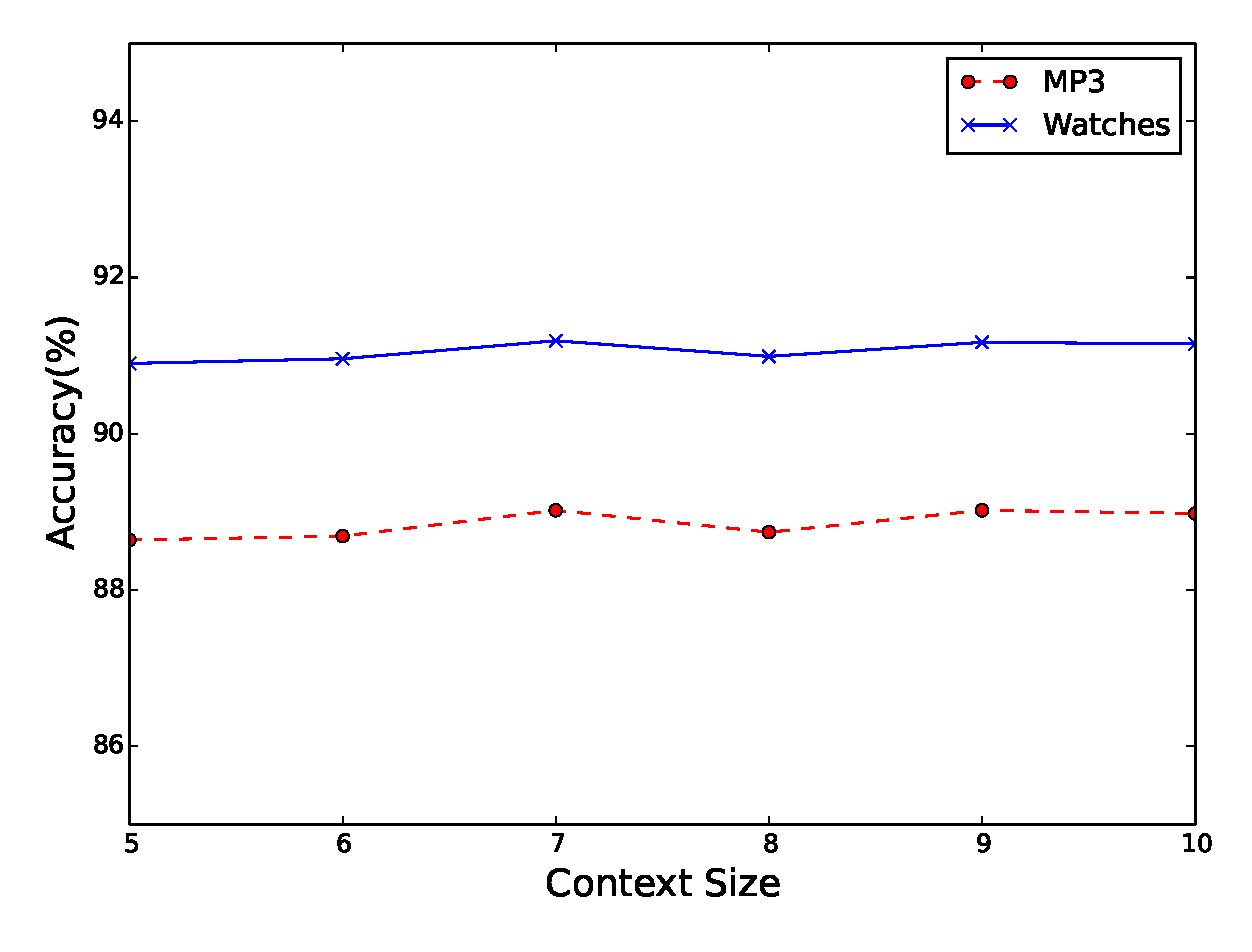
\includegraphics[width=140mm, height=110mm]{context_size.eps}
\caption{Variation of Accuracy with Different Context Size on Watches and MP3 Datasets. \label{fig:context_size}}
\end{figure}
We try to look how context size affects the accuracy on two amazon datasets, Watches and MP3.
Figure 5.2 depicts the accuracies obtained by varying the context size from 5 to 10. In both the cases, we find a peak at context size 7. There is an increase from 5 to 7 which denotes increase of context strength. As a result, we see increase in accuracies. Once the context size goes beyond a threshold, the semantic counterpart dominates which attains maximum at context size 10.\\
We also see that larger data size or training data affects the accuracy on test set. In this case, \emph{Watches} dataset is larger than \emph{MP3} dataset.\\

\section{SkipGram or CBOW}
SkipGram model tends to predict a context given a word whereas CBOW model predicts a word given a context. It seems intuitive and also from observation~\cite{Mikolov:13b} that SkipGram will perform better on semantic tasks and CBOW on syntactic tasks. We now try to evaluate how they differ on classification accuracies on the two datasets: \emph{Watches} and \emph{MP3}.
\begin{figure}[ht!]
\centering
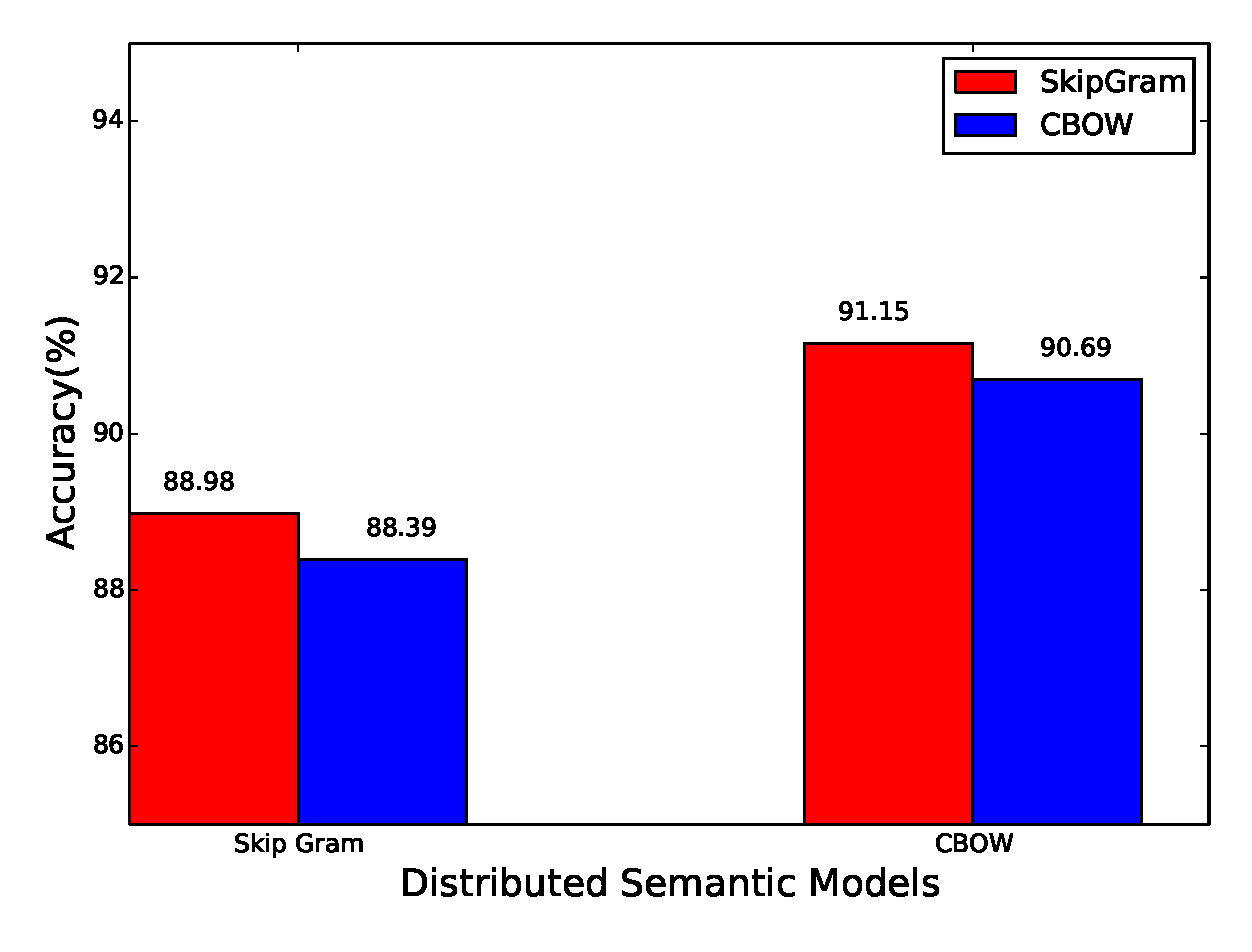
\includegraphics[width=140mm, height=110mm]{accuracy_sgcbow.eps}
\caption{Variation of Accuracy with skipgram and cbow on Watches and MP3 Datasets. \label{fig:accuracy_sgcbow}}
\end{figure}
Figure \ref{fig:accuracy_sgcbow} show that skipgram outperforms CBOW on sentiment classification task. It can be justified by the fact that sentiment inclination of a document is more oriented towards semantics of that document rather than just syntax and our results clearly demonstrate this fact.

\section{Skip-Gram and \emph{tf-idf} based Word Vectors}
In this experiment, we first generated $n$-dimensional word vectors by training skip-gram model on product and movie review corpus in Hindi and IMDB corpus in English. We then averaged-out word vectors for each document to create document vectors. This now acts as a feature set for that particular document.
We also created \emph{tf-idf} vectors for each document. This can be seen as a vector representation of that particular document. We then concatenated these document vectors with document vectors obtained after averaging-out word vector of each document.

In another experiment, we filtered out stop-words on the basis of their frequency in the corpus. Words which had very high or very low frequency were pruned as they had negligible contribution to the sentiment polarity of a document. This is a noise-reduction step and gives better results.

\section{Weighted Average Word Vectors}
Algorithm \ref{alg:weighted_average} presents a new approach to build document vectors using distributional semantics.Till date, everyone has ignored how to effectively use vector composition techniques and as a result, this area has seen very less attention. But we have successfully used \emph{idf} values to give weights to word vectors and hence obtain much better sentence/document vectors. Refer to \ref{sec:hindi_results} to see how this new technique has improved sentiment classification on Hindi reviews.\\

\RestyleAlgo{boxruled}
\LinesNumbered
\begin{algorithm}[H]
\large
\textbf{Skip-Gram}: Train skip-gram model on text to obtain word vectors.\\
\textbf{idf Calculation}: Calculate \emph{idf} value of each word with respect to given document (Refer \ref{subsec:tfidf}).\\
\textbf{Additive Composition}: For each document, $\sum_{i}(idf_i \times WordVector_i)$ is the document vector.\\
\textbf{Feature Set}: Repeat 3 for each document in training and test set to build document vectors.\\
\textbf{Classification}: Use a binary classification algorithm(SVM or Logistic Regression) to classify each test sample as positive or negative.
\caption{Weighted Average for Vector Composition}\label{alg:weighted_average}
\end{algorithm}
The advantage of this model is that once we obtain \emph{idf} values from training corpus, we can directly use it with test corpus without any additional computation.

\section{Word and Document Vectors with tf-idf: Enhanced Document Vectors}
This experiment redefined document representation in NLP used for sentiment classification. It has the property of including both syntactic and semantic properties of a piece of text. The limitations of skip-gram word vectors have been fulfilled by document vectors and hence we achieve state-of-the-art results on IMDB movie review dataset.

\section{Ensemble of RNNLM and Enhanced Document Vectors}
This experiment was done on IMDB movie review dataset. Here, we first trained a \emph{recurrent neural network} and then obtained predictions on test reviews in terms of probability. We trained another classier(Linear SVM) using Enhanced Document Vectors and then obtained predictions on test reviews. We then merged these two predictions using a simple heuristic, described below, to obtain final classification. This led to a tremendous increase in classification accuracy(Refer section \ref{sec:result}).\\
Let $y*$ be actual output and $y$ is the predicted output. The heuristic used is:
\begin{align}
((RNNLM_{pred}-1)*7+(0.5-SVM_{pred})).y<0 \text{  if } y*=1\\
((RNNLM_{pred}-1)*7+(0.5-SVM_{pred})).y<0 \text{  otherwise}
\end{align}

\section{Embeddings}
The quality of word vectors can be evaluated by comparing them with words which are closer to them semantically and syntactically. This is usually done via cosine similarity.
\begin{align}
similarity=cos(\theta)=\frac{A.B}{\|A\|\|B\|}=\frac{\sum_{i=1}^{n}A_i \times B_i}{\sqrt{\sum_{i=1}^{n}(A_i)^2}\times \sqrt{\sum_{i=1}^{n}(B_i)^2}}
\end{align}

Another evaluation can be done through tSNE~\cite{Maaten:08} which helps in visualization which maps each high-dimensional data point to a two or three-dimensional map. In our experiment, we took 5K words and plotted
them with tSNE (fig.~\ref{fig:5K_hindi}). 

\begin{figure}[H]
\centering
\includegraphics[width=140mm, height=110mm]{tsne.ps}
\caption{t-SNE visualization of the top 5000 Hindi Words in high dimensional space.  (Magnify to see details). \label{fig:5K_hindi}}
\end{figure}

Figure \ref{fig:5K_hindi_zoom} gives a closer look into few clusters which depicts the relation between words in high dimensional space. Figure \ref{fig:5K_hindi_zoom1} shows that words such as 
{\dn mO\8{j}d} and {\dn uplND} are closer to each other but farther from words such as {\dn \31EwyAdA} and {\dn aEDk}.

\begin{figure}[H]
    \centering
    \begin{subfigure}{.4\linewidth}
        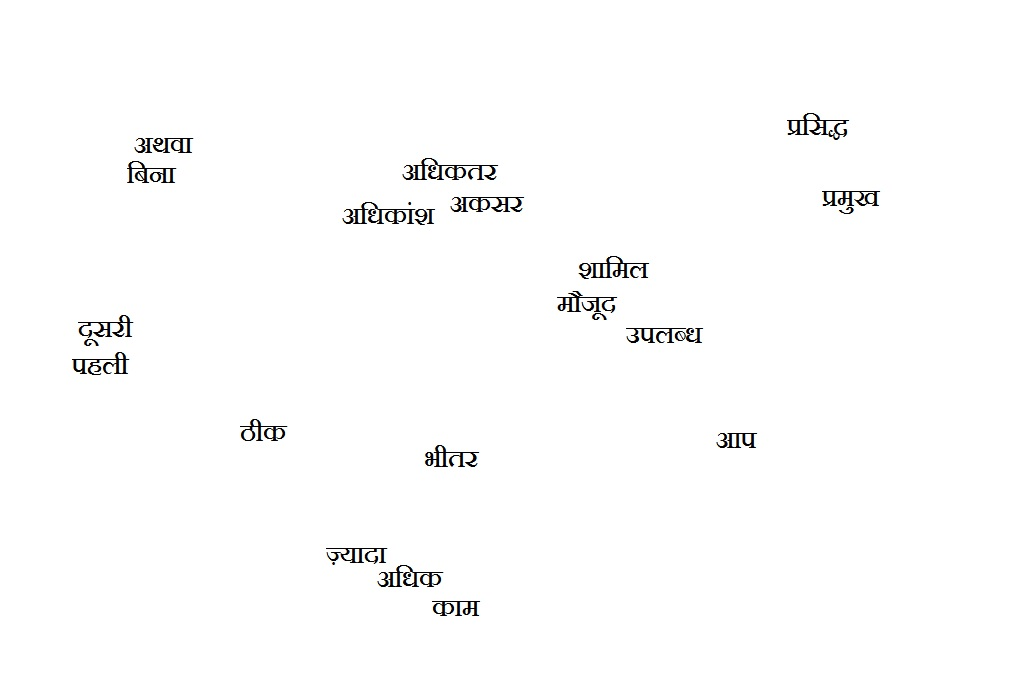
\includegraphics[scale=0.5]{5K_hindi_zoom1.eps}
        \caption{}
        \label{fig:5K_hindi_zoom1}
    \end{subfigure}
    \newline
    \begin{subfigure}{.4\linewidth}
        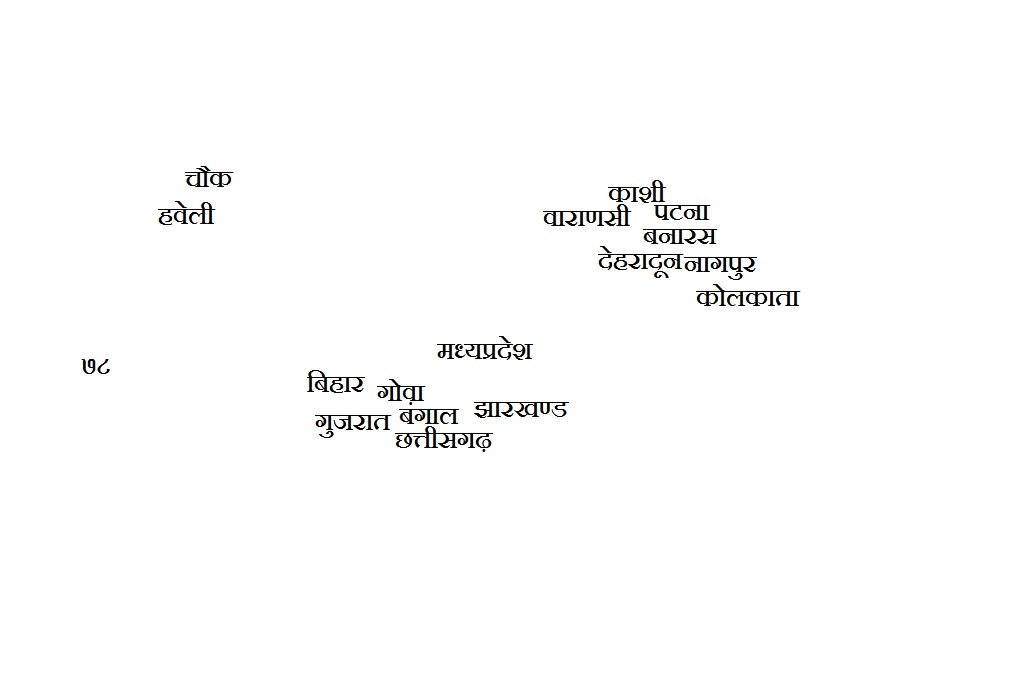
\includegraphics[scale=0.5]{5K_hindi_zoom2.eps}
        \caption{}
    \end{subfigure}
    \newline
    \begin{subfigure}{.4\linewidth}
        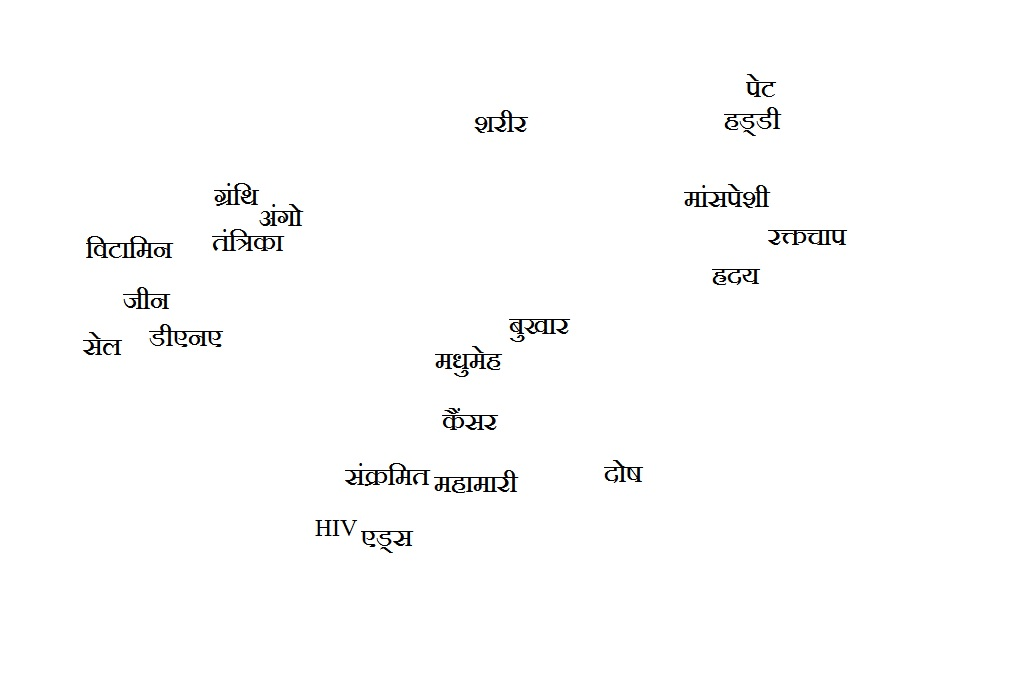
\includegraphics[scale=0.5]{5K_hindi_zoom3.eps}
        \caption{}
    \end{subfigure}
    \caption{A closer look at two clusters in the visualization showing a) quantity relations, b) locations and c) diseases.}
    \label{fig:5K_hindi_zoom}
\end{figure}


\section{Work Flow}
This section summarizes our approach in brief with graphics. This is a general classification system and includes building of enhanced document vectors.
\begin{figure}[H]
\centering
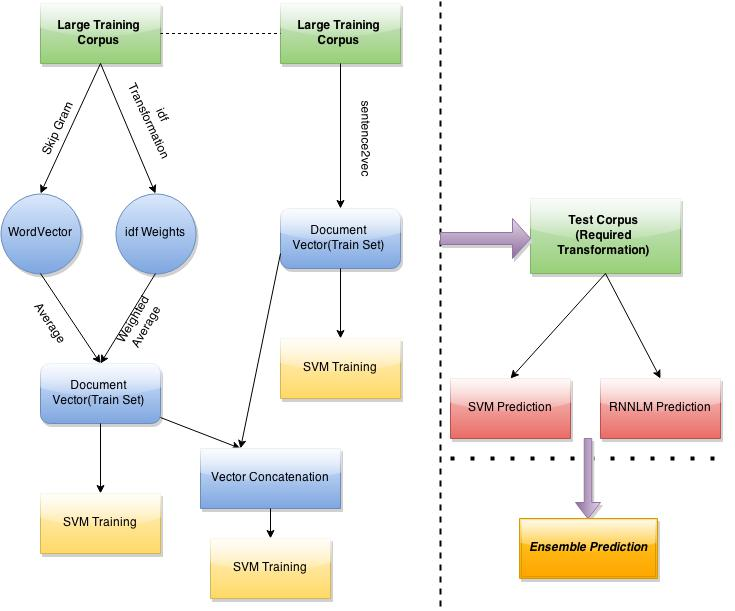
\includegraphics[width=160mm, height=180mm]{flow_chart.eps}
\caption{Work Flow Summary. \label{fig:flow_chart}}
\end{figure}

\section{Technical Specifications}
\subsection{Tools/Libraries}
\begin{itemize}
	\item Eclipse: An Integrated Development Environment helped speed up the process of coding and its subsequent debugging.
	\item Python: Being a very common and widely used programming language, loads of  documentation and third party libraries are available.
	\item Scikit: Open source library built on NumPy, SciPy and matplotlib which contains simple and efficient tools for data mining and data analysis.
	\item Gensim: It is an open-source vector space modeling and topic modeling toolkit, implemented in the Python programming language, using NumPy, SciPy and optionally Cython for performance. It is specifically intended for handling large text collections, using efficient online algorithms.
\end{itemize}

\subsection{System Requirements}
The code and tests have been successfully run on the following configuration. Any system with a configuration equal or higher than this should be able to do the job faster.
\begin{itemize}
	\item RAM: 16GB; fails to run on 8GB, due to the high amount of in memory data.
	\item CPU: Intel Core i7, 4th Generation; have used all 8 virtual cores with hyper-threading, with lower CPU, processes would take longer to complete.
	\item HDD: 1TB dedicated; Wikipedia Dump is the only component using considerable persistent memory. Storing pickle dumps of various datasets consumes considerable amount of memory.
\end{itemize}

	\chapter{Results}
\label{sec:result}
\section{Results on English Datasets}

\begin{table}[H]
\centering
\begin{tabular}{|c|c|c|c|}
\hline
\textbf{Method}                                                             & \textbf{IMDB}  & \textbf{Amazon} & \textbf{Hindi} \\ \hline
RNNLM (Baseline)                                               & 86.45          & 90.03           & 78.84          \\ \hline
Paragraph Vector \cite{Le:14}                                               & 92.58          & 91.30           & 74.57          \\ \hline
Averaged Vector                                                             & 88.42          & 88.52           & 79.62          \\ \hline
Weighted Average Vector                                                            & 89.56          & 88.63               & 85.90          \\ \hline
Composite Document Vector                                     & 93.91          & 92.17               & 90.30         \\ \hline
\end{tabular}
\caption {Comparison of accuracies on 3 Datasets(IMDB, Amazon Electronics Review and Hindi Movie Reviews(IITB)) for various types of document composition models. The state of the art for these tasks are: IMDB: 92.58\%~\cite{Le:14}; Amazon:85.90\%~\cite{Dredze:08}, Hindi:79.0\%~\cite{Bakliwal:12}.}
\label{table:3Datasets}
\end{table}
Table \ref{table:3Datasets} gives an overview of how our method compares against the earlier methods in sentiment analysis on3 different datasets. Even the word vector averaging seems to perform quite well when compared against complex baselines such as RNNLM.

\begin {table}[H]
\centering
\begin{tabular}{ | c | c | }
\hline
\textbf{Method} & \textbf{Accuracy} \\ \hline
Maas et al.(2011) & 88.89\\ \hline
NBSVM-bi (Wang \& Manning, 2012) & 91.22\\ \hline
NBSVM-uni (Wang \& Manning, 2012) & 88.29\\ \hline
SVM-uni (Wang \& Manning, 2012) & 89.16\\ \hline
Paragraph Vector (Le and Mikolov(2014)) & 92.58\\ \hline
WordVector+Wiki(Our Method) & 88.60\\ \hline
Weigted WordVector+TfIdf(Our Method) & 89.56\\ \hline
Weighted WordVector+TfIdf+Document Vector & \textbf{93.91}\\ \hline

\end{tabular}
\caption {Results on IMDB Movie Review Dataset}
\label{table:IMDB}
\end{table}

Table \ref{table:IMDB} summarizes the results obtained by others and by us on the IMDB movie review dataset. We have gone above the previous best~\cite{Le:14} by a margin of 1.33\% using enhanced document vector.

\begin {table}[H]
\centering
\begin{tabular}{ | c | c | }
\hline
\textbf{Method} & \textbf{Accuracy} \\ \hline
WordVector Averaging+TfIdf+Document Vector & 93.91\\ \hline
WordVector+TfIdf+Document Vector+RNNLM(Our Method) & \textbf{94.19}\\ \hline
\end{tabular}
\caption {Results on IMDB Movie Review Dataset}
\label{table:IMDB_rnnlm}
\end{table}

The main contributor for improvement in results is our enhanced document vector which overcomes the weaknesses of BOW and document vectors taken separately.\\
Table \ref{table:IMDB_rnnlm} is a further improvement in results once we incorporate predictions of RNNLM and enhanced document vector model together(voting ensemble).

Table \ref{table:IMDB_features} gives an overview of the results obtained with various experiments that we conducted on IMDB dataset. We have tried various vector composition models and feature composition models to obtain good results. Even a simple feature composition of word and document vector yield an improvement over the existing state-of-the-art suggesting that feature composition is a vital area when it comes to NLP tasks such as sentiment analysis.
\begin {table}[H]
\centering
\begin{tabular}{ | c | c | }
\hline
\textbf{Method} & \textbf{Accuracy} \\ \hline
WordVector Averaging & 88.42\\ \hline
Weighted WordVector Average & 89.56\\ \hline
Weigted WordVector Averaging+Wiki & 88.60\\ \hline
Weigted WordVector Averaging+TfIdf & 90.67\\ \hline
WordVector Averaging+Document Vector & 93.18\\ \hline
WordVector Averaging+Wiki+Document Vector & 93.18\\ \hline
WordVector Averaging+Document Vector+RNNLM & 93.70\\ \hline
WordVector Averaging+Wiki+Document Vector+RNNLM & 93.57\\ \hline
WordVector Averaging+TfIdf+Document Vector & 93.91\\ \hline
WordVector Averaging+Wiki+Document Vector+TfIdf & 93.55\\ \hline
WordVector Averaging+TfIdf+Document Vector+RNNLM & \textbf{94.19}\\ \hline
\end{tabular}
\caption {Comparison of results on IMDB Movie Review Dataset with Various Features}
\label{table:IMDB_features}
\end{table}

\begin{figure}[H]
\centering
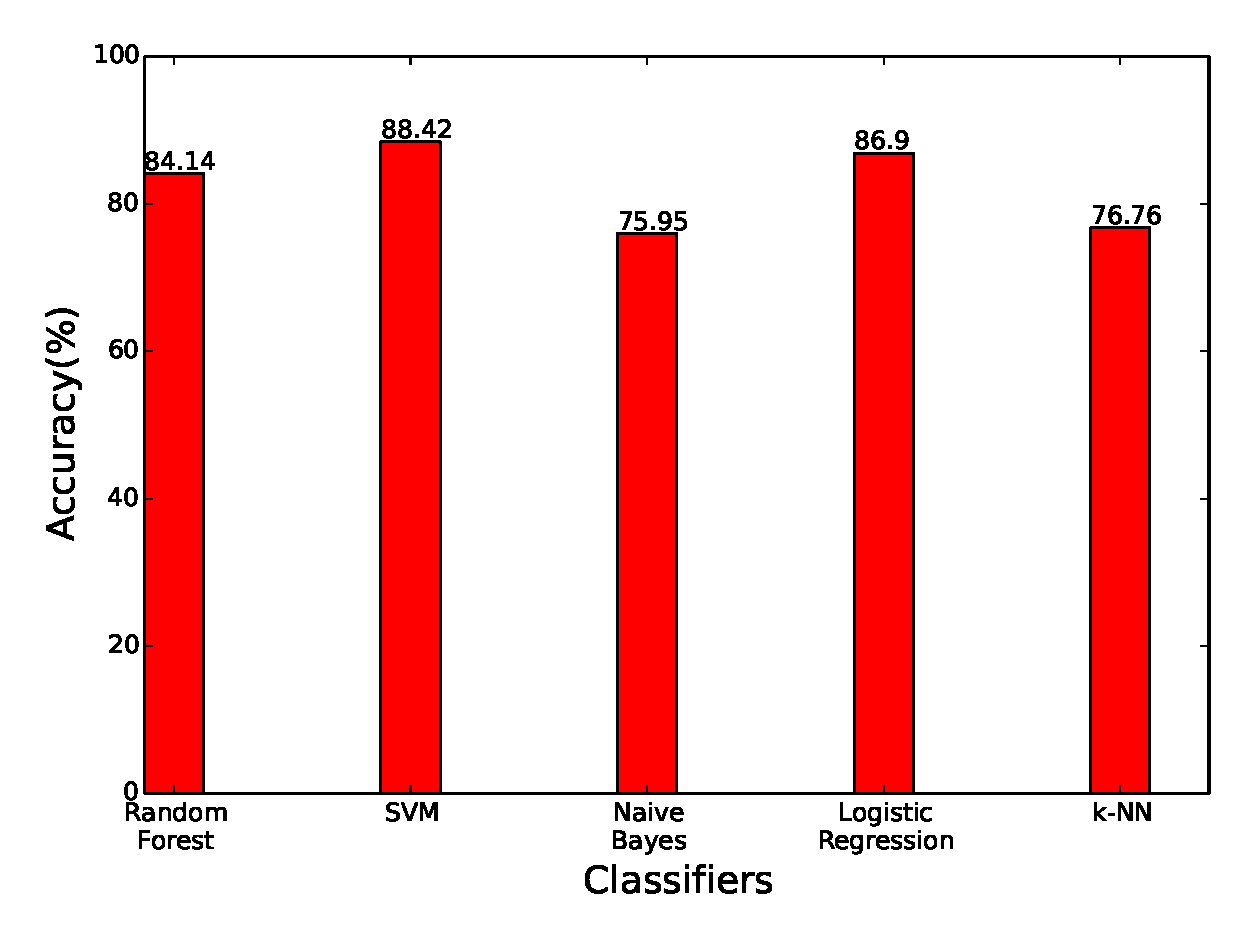
\includegraphics[width=140mm, height=120mm]{accuracy_wordvectors.eps}
\caption{Accuracies of Different Classifiers with Average Word Vectors(IMDB). \label{fig:accuracy_wordvectors}}
\end{figure}
Figure \ref{fig:accuracy_wordvectors} gives an overview of accuracies of various classifiers using word vector averaging method on IMDB dataset. This clearly gives a green signal to us for using Linear SVM as our classier in all experiments.

Table \ref{table:amazon} presents result of another experiment conducted on famous Amazon electronics review dataset(refer \ref{data:amazon}). Our vector averaging method alone has beaten previous best by 3.3\% which was based on maximum entropy method.
\begin {table}[H]
\centering
\begin{tabular}{ | c | c | }
\hline
\textbf{Features} & \textbf{Accuracy} \\ \hline
Dredze et al.(2008) & 85.90\\ \hline
Max Entropy & 83.79\\ \hline
WordVector Averaging (Our Method) & 89.41\\ \hline
Composite Document Vector (Our Method) & 92.17\\ \hline
Composite Document Vector + RNNLM & \textbf{92.91}\\ \hline
\end{tabular}
\caption {Results on Amazon Electronics Review Dataset}
\label{table:amazon}
\end{table}


\section{Results on Hindi Datasets}
\label{sec:hindi_results}
\begin {table}[h!]
\centering
\begin{tabular}{ | c | c |c | }
\hline
\textbf{Features} & \textbf{Accuracy(1)} & \textbf{Accuracy(2)} \\ \hline
WordVector Averaging & 78.0 & 79.62\\ \hline
WordVector+tf-idf & 90.73 & 89.52\\ \hline
WordVector+tf-idf without stop words & 91.14 & 89.97\\ \hline
Weighted WordVector & 89.71 & 85.90\\ \hline
Weighted WordVector+tf-idf & \textbf{92.89} & \textbf{90.30}\\ \hline
\end{tabular}
\caption {Accuracies for Product Review and Movie Review Datasets.}
\label{table:hindi_ourmethods}
\end{table}

Table \ref{table:hindi_ourmethods} represents the results using five different techniques for feature set construction. We see that there is a slight improvement in accuracy on both datasets once we remove stop-words but the major breakthrough occurs once we used weighted averaging technique for construction of document vectors from word vectors.

\begin {table}[h!]
\centering
\begin{tabular}{ | c | P{3cm} | c | }
\hline
\textbf{Experiment} & \textbf{Features} & \textbf{Accuracy} \\ \hline
Subjective Lexicon (Bakliwal et al., 2012) & Simple Scoring & 79.03\\ \hline
Hindi-SWN Baseline (Arora et al., 2013) & Adjective and Adverb presence & 69.30\\ \hline
Word Vector with SVM (Our method) & tf-idf with word vector & 91.14\\ \hline
Weighted Word Vector with SVM (Our method) & tf-idf+weighted word vector & \textbf{92.89}\\ \hline
\end{tabular}
\caption {Comparison of Approaches: Product Review Dataset}
\label{table:hindi_product}
\end{table}
Table \ref{table:hindi_product} and \ref{table:hindi_movie} compares our best method with various other methods which have performed well using techniques such as \emph{tf-idf}, subjective lexicon, etc.

\begin {table}[h!]
\centering
\begin{tabular}{ | c | P{3cm} | c | }
\hline
\textbf{Experiment} & \textbf{Features} & \textbf{Accuracy} \\ \hline
In language using SVM (Joshi et al., 2010)) & tf-idf & 78.14\\ \hline
MT Based using SVM (Joshi et al., 2010) & tf-idf & 65.96\\ \hline
Improved Hindi-SWN  (Bakliwal et al., 2012) & Adjective and Adverb presence & 79.0\\ \hline
WordVector Averaging & word vector & 78.0\\ \hline
Word Vector with SVM (Our method) & tf-idf with word vector & 89.97\\ \hline
Weighted Word Vector with SVM (Our method) & tf-idf+weighted word vector & \textbf{90.30}\\ \hline
\end{tabular}
\caption {Comparison of Approaches: Movie Review Dataset}
\label{table:hindi_movie}
\end{table}

Table \ref{table:hindi_neighbors} shows the top few similar words for certain words from the corpus with cosine similarity as a distance metric. The words which have higher cosine similarity tend to be semantically and syntactically related.
\begin {table}[ht!]
\centering
\begin{tabular}{ | c | c | c | }
\hline
\textbf{{\dn aQCA}} & \textbf{{\dn{KrAb}}} & \textbf{{\dn ByAnk}} \\ \hline
{\dn b\7{h}t} & {\dn EnrAsAjnk} & {\dn By\306wkr}\\ \hline
{\dn \7{s}pr} & {\dn kM)or} & {\dn BFqZ}\\ \hline
{\dn k\?vl} & {\dn nA\7{)}k} & {\dn ByAvh}\\ \hline
{\dn itnA} & {\dn bdtr} & {\dn avsAd}\\ \hline
\end{tabular}
\caption {Some sentiment words and their neighbors}
\label{table:hindi_neighbors}
\end{table}

\section{Odd One Out}
We trained Skip-Gram model on latest English and Hindi Wikipedia dump and tried to analyze the quality of embeddings by finding the odd word amongst a list of words. For this task, we took found cosine similarity between each pair and found the word with lowest cosine similarity with every other. The results are highlighted below-

\begin{table}[ht!]
\centering
\Large
\begin{tabular}{|l|l|l|l|}
\hline
breakfast         & \textbf{cereal} & lunch        & dinner  \\ \hline 
eight             & seven           & \textbf{owe} & nine    \\ \hline 
\textbf{shopping} & math            & reading      & science \\ \hline
\end{tabular}
\caption{Odd One Out in English}
\label{fig:english_odd}
\end{table}

\begin{table}[ht!]
\centering
\Large
\begin{tabular}{|l|l|l|l|}
\hline
{\dn BArt} & \textbf{{\dn \7{m}MbI}} & {\dn !s} & {\dn cFn}  \\ \hline 
{\dn lwkF}  & {\dn b\?hn} & \textbf{{\dn md\0}} & {\dn mEhlA}    \\ \hline 
\textbf{{\dn u\38Dwog}} & {\dn n\?tA}  & {\dn m\2/F} & {\dn srkAr} \\ \hline
\end{tabular}
\caption{Odd One Out in Hindi}
\label{fig:hindi_odd}
\end{table}

\section{Similar Words}
The trained skip-gram model was used for this task as well. We found the top few words which were closer in terms of cosine distance to the give word. The results are highlighted below-
\begin{table}[ht!]
\centering
\large
\begin{tabular}{|l|l|l|l|l|}
\hline
\textcolor{blue}{\textbf{Father}} & \textcolor{blue}{\textbf{France}} & \textcolor{blue}{\textbf{XBOX}} & \textcolor{blue}{\textbf{scratched}} & \textcolor{blue}{\textbf{megabits}} \\ \hline
grandfather & Germany & XBLA  & scraped & gigabits  \\ \hline 
uncle & French & Xbox360  & rubbed & kilobits  \\ \hline 
mother & Greece & SmartGlass  & bruised & megabit  \\ \hline 
father-in-law & Netherlands & 360/PS3  & cracked & terabits  \\ \hline 
brother & Scotland & XBLA   & discarded & MB/s  \\ \hline 
- & - & Qubed  & shoved & Tbit/s  \\ \hline 
- & - & Kinect  & tripped & -  \\ \hline 
\end{tabular}
\caption{Top Few Similar words in English}
\label{fig:english_similar}
\end{table}

\begin{table}[ht!]
\centering
\large
\begin{tabular}{|l|l|l|}
\hline
\textcolor{blue}{\textbf{{\dn BArt}}} & \textcolor{blue}{\textbf{{\dn \326wyApAr}}} & \textcolor{blue}{\textbf{{\dn aobAmA}}} \\ \hline
{\dn \3FEwd\?f} & {\dn \326wyvsAy} & {\dn E\3CAw\2Vn}  \\ \hline 
{\dn Et\3A9wt} & {\dn \7{p}nbF{\qvb}mA} & {\dn brAk} \\ \hline 
{\dn d\?f} & {\dn vAEZ>y} & {\dn sFn\?Vr} \\ \hline 
{\dn aA\1D\5\3FEwd\?f} & {\dn b\4{\qva}Ek\2g} & {\dn rA\6{\3A3w}pEt} \\ \hline 
{\dn l\38CwAK} & {\dn u\38Dwog} & {\dn uMmFdvAr} \\ \hline 
\end{tabular}
\caption{Top Few Similar words in Hindi}
\label{fig:hindi_similar}
\end{table}

	\chapter{Conclusions}

In this thesis, we have presented a new SMT interface called \texttt{z3.rkt},
which lets Racket programmers interact with an SMT solver programmatically. We
have demonstrated through examples the simplicity and usefulness of such an
interaction. The power of \texttt{z3.rkt} comes from the facilities provided
by Racket to build abstractions on top of the SMT-solving capabilities of Z3.
From the user's perspective, the integration is seamless and fully
transparent.

Our implementation is open source and freely available at
\begin{center}
\url{http://www.cse.iitk.ac.in/users/karkare/code/z3.rkt/}
\end{center}

\section{Scope for further work}

\texttt{z3.rkt}, like all large projects, is a work in progress. What has been
implemented as of the writing of this thesis is a useful subset of Z3
functionality, but there are several gaps still to be filled:

\begin{itemize}
\item Supporting more Z3 constructs, including bit-vectors and external theories
\item Deriving new abstractions guided by practical use cases
\item Possibly integrating with other SMT solvers
\end{itemize}

In the long term, we hope the community will find this system useful and will
contribute to the project to solve large practical problems.

	
%	\appendix 
%	\chapter{Development Details}

%	\section{Last.FM APIs}
%		An api-key is required for calling the api. This can be obtained by creating a developer account on their website.
		
%		Base URL: http://ws.audioscrobbler.com
%\begin{itemize}
%	\item Recent Tracks: URL: /2.0/?method=user.getrecenttracks\&user=<user>\&api\_key=<api\_key>\&format=<format>
%		<user>: The user for which the history is to be fetched.
%		<api\_key>: Obtained from their developer's portal.
%	\item Top Tags: 
%\end{itemize}
	
	\backmatter
	\doublespacing
	
	\addcontentsline{toc}{chapter}{Bibliography}
	\bibliographystyle{plain}
	\bibliography{references}
\end{document}
